\documentclass{article}
\usepackage{iclr2027_conference,times}
\usepackage[T1]{fontenc}
\usepackage[utf8]{inputenc}
\usepackage{amsmath,amssymb,amsfonts}
\usepackage{booktabs}
\usepackage{multirow}
\usepackage{graphicx}
\usepackage{microtype}
\usepackage[table]{xcolor}
\definecolor{failorange}{HTML}{C16E71}
\definecolor{wsblue}{HTML}{6E8FB2}
% --- exemplar-style table/writing toolkit, rendered in the paper's muted palette ---
\definecolor{gain}{HTML}{4E8A6B}   % readable sage green (same family as figure sage #7DA494)
\definecolor{loss}{HTML}{B5545A}   % readable muted terracotta (same family as V/rose #C16E71)
\definecolor{deltaz}{gray}{0.55}   % neutral for negligible change
\newcommand{\dgain}[1]{\,\textcolor{gain}{\scriptsize #1}}   % small green delta, append after a number
\newcommand{\dloss}[1]{\,\textcolor{loss}{\scriptsize #1}}   % small terracotta delta
\newcommand{\dzero}[1]{\,\textcolor{deltaz}{\scriptsize #1}} % small neutral delta
\definecolor{wsRow}{HTML}{EEF3F8}  % very light steel-blue tint for the workspace/method row
\definecolor{refRow}{gray}{0.955}  % very light gray for reference / oracle / diagnostic rows
\newcommand{\wsrow}{\rowcolor{wsRow}}
\newcommand{\refrow}{\rowcolor{refRow}}
\newcommand{\myparagraph}[1]{\vspace{2pt}\noindent\textbf{#1}\ }
\usepackage{longtable}
\usepackage{float}
\usepackage{algpseudocode}
\usepackage{soul}
\usepackage[colorlinks=true,linkcolor=blue,citecolor=blue,urlcolor=blue]{hyperref}

% Compatibility for the local TeX Live array/colortbl version pair.
\makeatletter
\@ifundefined{insert@pcolumn}{\let\insert@pcolumn\insert@column}{}
\makeatother

% Yellow revision markup for the incremental experimental update.
% Change \showupdatestrue to \showupdatesfalse for a clean copy.
\newif\ifshowupdates
\showupdatestrue
\sethlcolor{yellow}
\ifshowupdates
  \newcommand{\updated}[1]{\hl{#1}}
  \newcommand{\updatednum}[1]{\colorbox{yellow!55}{\strut #1}}
  \newcommand{\updatedrow}{\rowcolor{yellow!25}}
  \newcommand{\updatedparagraph}[1]{\par\smallskip\noindent\colorbox{yellow!20}{\parbox{\dimexpr\linewidth-2\fboxsep\relax}{#1}}\par\smallskip}
\else
  \newcommand{\updated}[1]{#1}
  \newcommand{\updatednum}[1]{#1}
  \newcommand{\updatedrow}{}
  \newcommand{\updatedparagraph}[1]{#1}
\fi

\newcommand{\Wrr}{\ensuremath{W}}
\newcommand{\Vrep}{\ensuremath{V}}
\newcommand{\Ms}{\ensuremath{M_s}}

\title{Remember What You Thought, Not What You Said:\\
Workspace-Gated Episodic Memory for LLMs}
\author{Anonymous authors}
\date{}

% Uncomment only for the camera-ready version.
% \iclrfinalcopy
\begin{document}
\maketitle

\begin{center}
\itshape ``We can know more than we can tell.''\\[2pt]
{\upshape --- Michael Polanyi, \emph{The Tacit Dimension} (1966)}
\end{center}
\vspace{4pt}

\begin{abstract}
Memory-limited LLM agents decide what to store by asking the model what is
important, the self-rated importance scores introduced by Generative Agents
and inherited by most agent memory systems. Under experimental control of
content provenance, we show this practice fails exactly where memory matters
most: information the model inferred while reading but never wrote down. On
sparsely cued construct-valid benchmarks, verbal importance ratings fall at
or below chance as a ranking signal, while the same models demonstrably carry
the inferred content. A training-free workspace readout of the residual
stream, derived from the J-lens construction, recovers it on one-hop designs
and causally patching the corresponding directions flips memory-based answers
where sham directions do not ($0.70$ vs.\ $0.05$ at 7B,
$p{=}2.4\times10^{-4}$). \updated{Under a corrected log-space verbal-score
definition, the Decoupled workspace--report gap is $+0.1526$ to $+0.3135$
across four capable-scale model families, with every paired confidence
interval excluding zero.} The model knows more than it tells, so we gate
memory on what it knows: a training-free write gate scores candidates with
the workspace readout at zero additional probe passes and reaches the
selection-oracle accuracy on the primary construct-valid cell.
\updated{The reporting channel is repairable at scale: workspace-derived
self-distillation raises Qwen3-8B verbal AUC by $+0.2128$ on average across
three locked seeds while changing workspace AUC by less than $0.001$. A
separate, probe-blind RL-QA policy repairs the action interface, improving
budget-2 recall by $+5.88$ to $+8.82$ percentage points across three Qwen3-8B
seeds.} Agents should remember what they thought, not what they say they
thought.
\end{abstract}

\section{Introduction}
\label{sec:intro}

An LLM agent that operates over days cannot keep everything in context. Since
Generative Agents \citep{park2023generative}, the standard answer to the question of what to store has been to ask the model
itself: rate the importance of each candidate memory and keep the top-rated
ones. Variants of this reflection-based admission
control run inside most deployed agent memory stacks
\citep{packer2023memgpt, zhong2023memorybank}. The practice rests on an assumption that has never been tested under
experimental control of content provenance: that a model's verbal report of
what is important tracks what will actually be useful.

We test this assumption under experimental control of content provenance and
find that it fails for the content that memory selection most needs to capture. We construct episodic
benchmarks in which the single most useful item is either (i) stated explicitly in
the text, or (ii) a silent inference: a bridge concept (``the city is Madrid'') that the model can be shown to carry while reading (\S\ref{sec:causal}) but that never appears
as a word and is required only later, when a probe question arrives (in the
construct-valid designs the bridge is also never the answer itself,
\S\ref{sec:setup}). Asked which concepts are worth remembering, models at every scale we tested
(0.5B--7B) and at every post-training stage (SFT, DPO, RLVR) confidently
nominate vivid, useless surface words and reject the silent bridge: on the
sparse-cue construct-valid benchmarks, verbal importance is at or below
chance as a ranking signal (AUC $0.17$--$0.49$; Table~\ref{tab:master};
Fig.~\ref{fig:hero}). The same reports are good when the useful content is
explicit, better there than any internal signal we test. The failure is robust to probe wording, to the canonical 1--10 rating form,
and to letting the model deliberate before answering; its one measured
boundary is cue density, summarized in \S\ref{sec:dissociation} and mapped
in Appendices~\ref{app:vrobust} and~\ref{app:replications}.

The model knows more than it tells: the information is present in its
internal state but not in its report.
Building
on the J-lens ``workspace'' construction of \citet{anthropic2026workspace}, we read
each concept's availability directly off the residual stream at the end of
encoding: the peak reciprocal rank of the concept's token across layers under the
logit lens \citep{nostalgebraist2020logitlens}. This readout ranks the silently inferred bridges that self-report rejects
above the competing candidates (AUC $0.62$--$0.67$ at 7--8B across four model
families, including the latest Qwen3), is not explained by surface presence, embedding relevance, or
prompt wording (App.~\ref{app:vrobust}), and is causally load-bearing: steering the
bridge's input-side direction while the model answers from memory changes the
answer far more often than a sham direction ($0.70$ vs.\ $0.05$ flip rate at
7B at the gentlest tested scale, $0.60$ vs.\ $0.10$ at 3B;
Table~\ref{tab:causal}).

\updatedparagraph{Downstream, gating memory on the workspace score costs zero
probe passes. The workspace-only arm reaches the selection-oracle accuracy at
7B on the construct-valid benchmark ($0.525$ vs.\ $0.525$) and reaches $0.75$
recall-QA at 0.5B on Evoked. These workspace and oracle arms do not consume
the migrated verbal score; historical direct comparisons against verbal
selected sets are retained as prior evidence and are not used as corrected-v3
headline claims. Full policy comparisons are in \S\ref{sec:prgresults}.}
Finally, the failure is repairable: the reporter never learned to read the
workspace. \updated{On Qwen3-8B, self-distillation from frozen workspace
rankings increases held-out Decoupled verbal AUC by $+0.1642$, $+0.2868$, and
$+0.1873$ across three independently locked seeds (mean $+0.2128$), while
workspace AUC changes by less than $0.001$. Separately, a probe-blind RL-QA
objective learns the admission decision directly from future QA utility and
improves budget-2 recall by $+5.88$ to $+8.82$ points across the same three
8B seeds.} These two additions repair different interfaces: what the model
says is worth remembering, and what the agent actually stores.

\updatedparagraph{\textbf{Revision scope.} The original architecture,
training-free workspace gate, causal intervention, mechanism analyses, and
figures are retained. The new experiments add a corrected 24-checkpoint
log-space measurement grid, a five-size Qwen3 scale ladder, multi-seed
Qwen3-8B Alignment and RL-QA, and exploratory 14B/32B boundary runs. Updated
v3 tables supersede the corresponding pre-migration verbal-score numbers;
workspace-only causal and gating arms are unaffected.}

\textbf{Contributions.}
\textbf{(1)}~A content-provenance regime map for LLM introspective salience:
verbal importance reports are reliable for explicit content and fall at or
below chance for construct-valid silently inferred content, replicated across
four model families (including the latest Qwen3 generation) and three probe wordings, with episode-cluster bootstrap
statistics and a machine analogue of metacognitive efficiency
(\S\ref{sec:setup}, \S\ref{sec:results}). We release the four
provenance-controlled benchmarks, show that existing naturalistic benchmarks
structurally cannot exercise the silently inferred regime
(App.~\ref{app:locomo}), and map the regime's boundary with a measured
cue-density analysis across three generators (App.~\ref{app:replications}).
\textbf{(2)}~A training-free workspace write gate, the first use of a
J-lens-style readout as a write-admission signal, with causal evidence that
memory-based answers read the patched workspace content and budgeted-recall
payoff up to selection-oracle level at zero probe cost; a provenance-routed
extension (PRG) covers mixed streams at tight budgets (\S\ref{sec:method},
\S\ref{sec:prgresults}).
\textbf{(3)}~A post-training diagnosis: in our stage sweep, none of 11 transitions
(8 Qwen base$\to$instruct pairs; OLMo-2 SFT$\to$DPO$\to$RLVR) improves the
workspace channel, and the verbal channel's miscalibration, already present in
raw-probed base models, persists or worsens; we propose and validate
metacognitive alignment, a self-distillation procedure that repairs the verbal
channel, in two model families (\S\ref{sec:extensions}).
\textbf{(4)}~A boundary analysis showing what the static workspace does and does
not hold: a trained future-token lens cannot rescue compositional (two-hop)
bridges, but a utility-gradient readout, the infinitesimal version of our
causal intervention, can in the Qwen family (paired $+0.125$ over the static
readout at 7B; family-dependent, \S\ref{sec:extensions},
App.~\ref{app:family}).
\updatedparagraph{\textbf{(5)}~A scaled and multi-seed extension that separates two
repair targets: workspace-derived self-distillation calibrates the verbal
reporter, whereas probe-blind RL-QA learns the memory action without observing
the workspace probe (\S\ref{sec:newexperiments}).}

\begin{figure}[t]
\centering
\IfFileExists{figures/intro.png}{%
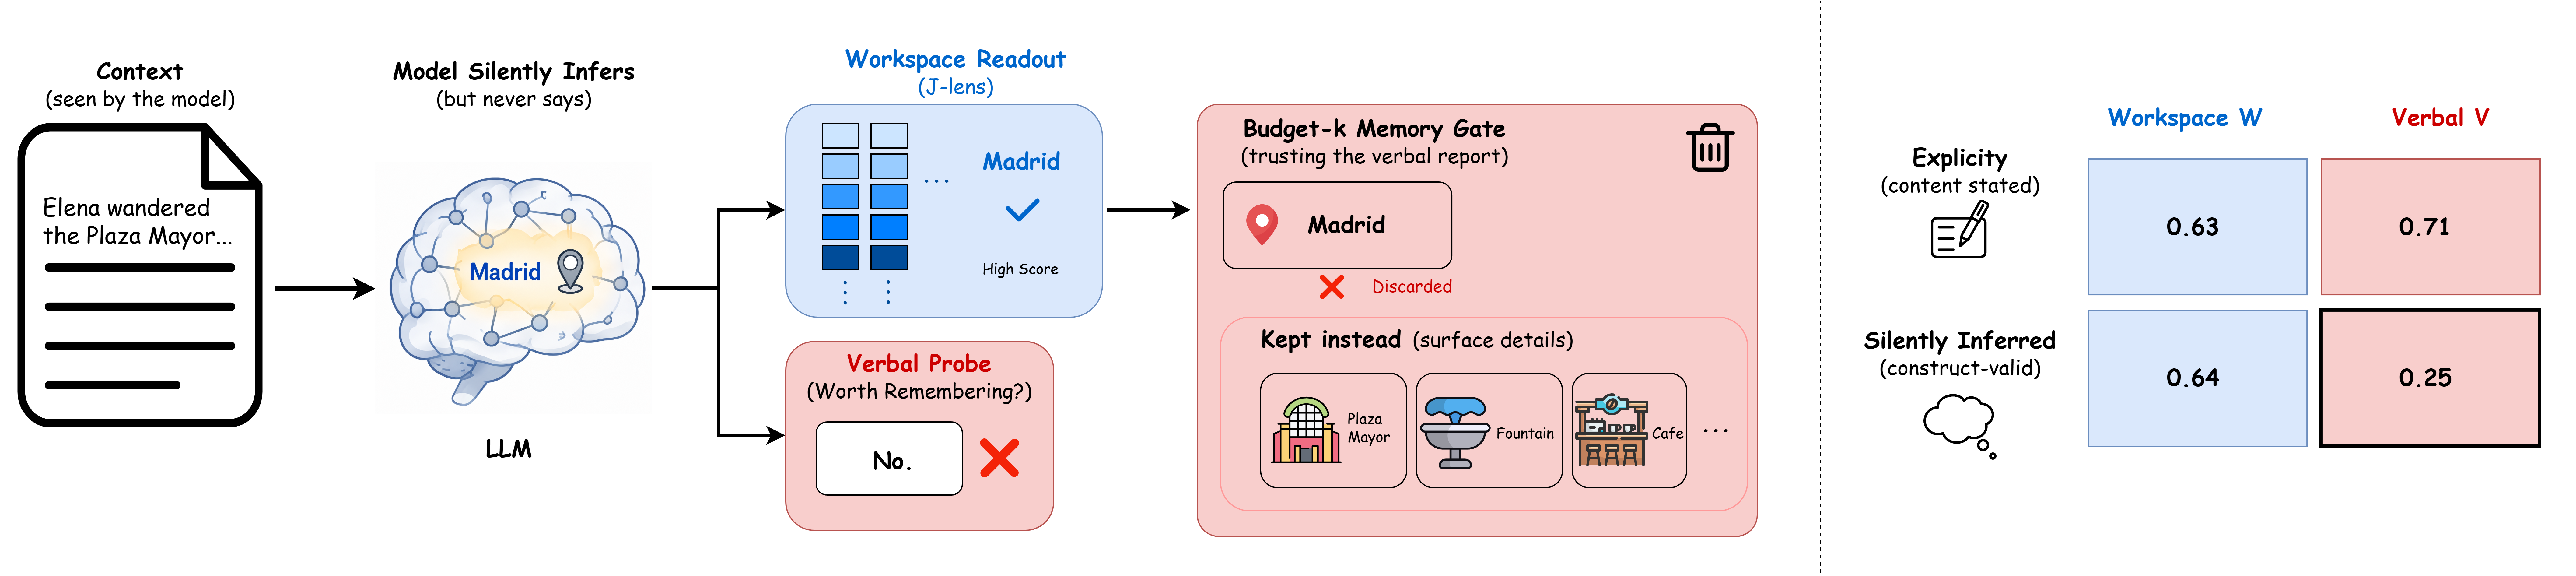
\includegraphics[width=\textwidth]{figures/intro.png}}{%
\fbox{\parbox[c][4.6cm][c]{0.96\textwidth}{\centering
\emph{Hero figure (figures/fig1\_hero.pdf).}\\[4pt]
\textbf{Left:} write-gating schematic. Context ``Elena wandered the Plaza
Mayor\ldots'' $\rightarrow$ model silently infers \emph{madrid} (high in the
J-lens workspace readout $\checkmark$) but rates it unimportant verbally
($\times$) $\rightarrow$ budget-$k$ gate on the verbal report drops the item
needed for ``What language should Elena use?''.\\[4pt]
\textbf{Right:} $2\times2$ AUC heatmap, regime (explicit / inferred)
$\times$ channel (workspace $W$ / verbal $V$), showing the dissociation:
$V$ wins on explicit, is anti-calibrated on inferred; $W$ the reverse.}}}
\caption{\textbf{Left:} the write-gating problem. Reading ``Elena wandered the
Plaza Mayor\ldots'', the model silently infers \emph{madrid}, and the inference
is visible in a J-lens-style workspace readout of its residual stream; asked
whether \emph{madrid} is worth remembering, it confidently says no. A budget-$k$ memory gate
that trusts the verbal report discards exactly the item needed to answer ``What
language should Elena use?''. \textbf{Right:} AUC of each channel at identifying
truly load-bearing items (Qwen-3B shown; same qualitative dissociation at
3B--7B in all four families, with knife-edge small-scale cells noted in
App.~\ref{app:prereg};
Table~\ref{tab:master}): the verbal report is good for explicit content but
below chance for construct-valid silently inferred content (boxed cell;
generator analysis in \S\ref{sec:dissociation}); the workspace readout is
not.}
\label{fig:hero}
\end{figure}

\section{Background and Related Work}
\label{sec:related}

\paragraph{Importance and memory admission.}
Generative Agents combines an importance rating with recency and
relevance for retrieval \citep{park2023generative}. MemoryBank, MemGPT,
Mem0 and A-MEM provide persistence, memory operations and organization
\citep{zhong2023memorybank,packer2023memgpt,mem0,amem2025}.
Admission methods use externally supplied utility signals: A-MAC
combines LLM assessment with textual support and memory attributes
\citep{amac2026}, a multi-factor value model optimizes evidence retention
\citep{valuemodel2026}, and Causal Memory Intervention scores answers to
a known request under memory interventions \citep{cmi2026}.
SDA derives admission targets from the host model's own computation
before a future request is available. Our provenance controls show how
importance reports prioritize passage content during this decision.
The controlled admission tests
complement long-conversation evaluations such as LoCoMo and LongMemEval
\citep{maharana2024locomo,wu2025longmemeval}.

\paragraph{Learned memory management.}
Learned memory management spans admission, control of memory operations
and distillation of experience. ConsistencyGate \citep{consistencygate2026}
is a write-time admission gate that filters candidates by self-consistent
support in the source context. Nemori \citep{nemori2026} distills
interaction sequences into memory using prediction error and shares the
motivation that heuristic importance scores encode designer intuition.
MemCon \citep{memcon2026} models retrieval, consolidation and forgetting as
a learned control policy. AgeMem \citep{agemem2026} exposes memory
operations as tool actions trained with reinforcement learning. TMEM
\citep{tmem2026} writes distilled experience into low-rank weights instead
of an external store. Agent Memory Distillation \citep{amd2026} transfers a
larger teacher agent's trajectories into structured memory for a smaller
student. The survey of \citet{hu2025memorysurvey} provides broader context
for these memory systems. SDA addresses the admission decision for a single
passage before any future request, with supervision from the same model's
internal rankings rather than support in the context, prediction error,
task reward or a larger teacher. Its self-distillation occurs within one
model, distinguishing it from teacher-to-student memory distillation.

\paragraph{Internal signals and representation readouts.}
EM-LLM, SirLLM and Titans use surprisal, entropy and gradient-based
surprise for memory \citep{fostiropoulos2024emllm,yao2024sirllm,behrouz2025titans}.
SDA turns internal candidate rankings into admission supervision.
The workspace readout builds on the logit lens and J-lens
\citep{nostalgebraist2020logitlens,anthropic2026workspace}; tuned lenses,
Future Lens and Patchscopes also decode internal representations
\citep{belrose2023tuned,pal2023futurelens,ghandeharioun2024patchscopes}.
SDA uses these measurements offline to train a served language interface.

\paragraph{Self-distillation and internal information.}
Knowledge distillation transfers teacher predictions to a student,
including between models of the same architecture
\citep{hinton2015distilling,furlanello2018bornagain}. SDA transfers a
frozen model's rankings into its own importance prompt.

Internal states can predict correctness beyond expressed confidence
\citep{kadavath2022know,azaria2023internal,orgad2024llmsknow}, and stated
reasoning can omit influences on an answer \citep{turpin2023cot}.
Salience can likewise be poorly reported \citep{trienes2025salience};
introspection training teaches models to predict their own behavior
\citep{binder2024introspection}. SDA makes this transfer serve a
prospective decision: admit a concept before the question that uses it.

\section{Evaluation Setup}
\label{sec:setup}
\label{sec:problem}

Given a passage $x$ and ordered candidates $C=(c_1,\ldots,c_m)$,
admission stores $K\subseteq C$ with $|K|\leq k$. The future question
$q$ and answer $a$ are hidden. When $q$ arrives, the frozen reader sees
only $q$ and $K$; the original passage has left its window. Every policy
receives the same candidates and budget. We measure three successive
outcomes: candidate ordering, retained information and answer correctness.

\paragraph{Ranking within the episode.}
Within-episode area under the receiver operating characteristic curve
(AUC) is the fraction of useful--distractor pairs ordered correctly,
with half credit for ties, averaged across episodes. For useful concept
$b_i$ in episode $i$, score $s$ and $n$ episodes,
\begin{equation}
A_{\mathrm{episode}}
=\frac{1}{n}\sum_{i=1}^{n}\frac{1}{|C_i|-1}
\sum_{c\in C_i\setminus\{b_i\}}
\left[\mathbf{1}\{s(b_i)>s(c)\}
+\tfrac12\mathbf{1}\{s(b_i)=s(c)\}\right].
\label{eq:episodeauc}
\end{equation}
It measures the ordering among concepts that actually compete for memory. Pooled AUC
instead compares candidates across the entire battery and summarizes
score discrimination. Retention at budget $k$ connects this ordering
to the admitted set. For the provenance analysis,
we replace utility labels with statedness labels and report
\emph{provenance AUC}: discrimination of stated from unstated candidates
under a case-insensitive stem match against the passage.

\paragraph{Retention of the useful concept.}
Bridge retention is the fraction of episodes whose stored set contains
the construction-labelled useful concept:
\begin{equation}
B_k=\frac{1}{n}\sum_{i=1}^{n}\mathbf{1}\{b_i\in K_i\}.
\label{eq:retention}
\end{equation}
It directly measures what
survives the budget; correct answering additionally depends on the
reader and the other stored concepts. An oracle-label policy prioritizes
the intended bridge and provides a reference for this construction.

\paragraph{Downstream recall.}
Recall is the fraction of future questions answered correctly from
stored concepts by the frozen reader. It measures the downstream effect
of admission for a fixed reader. A policy can rank the bridge
above most distractors yet drop it at a small budget; a retained bridge
can still lead to an incorrect answer. Reporting all three outcomes
locates these distinct transitions from score to memory to answer.
The reader answers greedily, with Qwen3 thinking disabled. A blind
semantic judge receives only the question, gold answer and response;
it accepts a committed correct answer or exact equivalent. A separate
string-match grader checks agreement (App.~\ref{app:judge}).
Question-only and whole-passage readers establish how much the answer
can be recovered before admission and with the complete original input.

\paragraph{Comparisons.}
Baselines are the untrained yes/no importance report, a 1--10 importance
rating, reversed yes/no report, admit what the passage omits,
omission then report, wording variants, the provenance-adjusted report,
the combined teacher used directly, random selection, output likelihood,
the workspace readout, and students trained from either teacher signal
alone. All receive the passage with the future question hidden
(App.~\ref{app:baselines}). Paired AUC differences use 4,000-draw
whole-episode bootstraps and 95\% intervals; recall comparisons use
exact McNemar tests on paired answers and seed-averaged differences
with paired 95\% bootstrap intervals (Table~\ref{tab:paired}). Trained results give three-seed
means and sample standard deviations. Bold table entries identify SDA.

\paragraph{Evaluation scale.}
\label{sec:breadth}
\label{sec:models}

The principal diagnostic comparison covers eight models from four
families: Qwen2.5-7B, OLMo-2-7B, Mistral-7B and Qwen3 at 1.7B, 4B,
8B, 14B and 32B
\citep{qwen2025,olmo2,jiang2023mistral,qwen3}. The extended grid contains
23 checkpoints across those families and GPT-2, including base and
post-training stages (App.~\ref{app:breadth}). SDA trains three seeds
for each of six models: Qwen3-8B, 14B and 32B and the other three
7B families, totaling 18 principal training runs. Each supplies its
own teacher, adapter and frozen reader.

Training and validation contain 175 and 45 episodes, drawn from
88 Explicit episodes and 132 implied-answer episodes, including the
57-episode alternate-author benchmark. In an implied-answer episode,
the passage cues an unstated useful concept that itself supplies the
answer; Decoupled instead requires a further inference from that concept. Development uses Decoupled
(68 episodes), Compositional (52), and two separate 68-episode pools
that add confusable or unrelated unstated distractors to Decoupled.
Fresh-1 and Fresh-2 contain 316 and 363 episodes; the entity-bridge
benchmark contains 42. Fresh-2 passage and pool controls reuse its
363 episodes. Budgets are $k=1,2,3$; the main comparison uses the
statedness-balanced pool, with $k=2$ reported across all six models.
The paired Fresh-2 grading audit totals 13,068 answers across the
18 SDA--report comparisons; both graders evaluate every answer.



\section{Self-Distilled Admission}
\label{sec:method}

SDA distills a frozen model's candidate rankings into yes/no admission
judgments, training the importance interface to retain useful inferences
(Fig.~\ref{fig:sda}).

\begin{figure*}[t]
\centering
\begin{tikzpicture}[
  font=\small,
  box/.style={draw=wsblue,fill=wsblue!9,rounded corners=2pt,
    align=center,minimum height=11mm,inner sep=4pt},
  report/.style={box,draw=failorange,fill=failorange!9},
  arr/.style={-{Stealth[length=2mm]},semithick,draw=wsblue!85!black}
]
\node[anchor=west,font=\small\bfseries] at (0,0)
  {(a) Training: offline, once};
\node[box,text width=25mm] (inputs) at (1.4,-0.95)
  {Context $x$\\Candidates $C$};
\node[box,text width=31mm] (readouts) at (5.0,-0.95)
  {Frozen teacher\\$W(c;x)$ and LL$(c;x)$};
\node[box,text width=23mm] (teacher) at (8.6,-0.95)
  {Rank mean\\$T(c;x)$};
\node[report,text width=22mm] (labels) at (11.6,-0.95)
  {Top-2\\yes/no labels};
\node[report,text width=48mm] (student) at (6.5,-2.35)
  {Train the SDA adapter\\on the admission prompt};
\draw[arr] (inputs) -- (readouts);
\draw[arr] (readouts) -- (teacher);
\draw[arr] (teacher) -- (labels);
\draw[arr] (inputs.south) |- (student.west);
\draw[arr] (labels.south) |- (student.east);

\node[anchor=west,font=\small\bfseries] at (0,-3.5)
  {(b) Deployment: standard serving};
\node[box,text width=25mm] (serveinputs) at (1.4,-4.4)
  {Context $x$\\Candidates $C$};
\node[report,text width=31mm] (sda) at (5.0,-4.4)
  {Admission prompt\\+ SDA adapter};
\node[box,text width=23mm] (memory) at (8.6,-4.4)
  {Top-$k$\\memory store};
\node[box,text width=22mm] (reader) at (11.6,-4.4)
  {Frozen reader\\answers $q$};
\node[anchor=north,align=center,font=\scriptsize] at (reader.south)
  {Future question $q$\\arrives at recall};
\draw[arr] (serveinputs) -- (sda);
\draw[arr] (sda) -- (memory);
\draw[arr] (memory) -- (reader);
\end{tikzpicture}
\caption{\textbf{SDA training and deployment.} (a) The frozen teacher labels
the top-2 candidates from context $x$ and candidate set $C$.
(b) The trained adapter selects the top-$k$ concepts for the frozen
reader; the future question enters at recall.}
\label{fig:sda}
\end{figure*}


\subsection{A teacher from the model's own computation}
\label{sec:teacher}

\paragraph{Workspace readout.}
Let $h_\ell(x)\in\mathbb{R}^d$ be the residual state at the final context
position after transformer layer $\ell$, with $L$ layers in total.
Final normalization $\mathrm{LN}$ and unembedding $W_U$ give vocabulary
logits $z_\ell(x)=W_U\,\mathrm{LN}(h_\ell(x))$.
Writing $\mathrm{rank}_\ell(t)=1+|\{v:z_{\ell,v}>z_{\ell,t}\}|$, the
workspace readout is the peak reciprocal rank across layers and
first-token forms:
\begin{equation}
W(c;x)=\max_{1\leq\ell\leq L}\;\max_{t\in T(c)}
\frac{1}{\mathrm{rank}_\ell(t)}.
\label{eq:wrr}
\end{equation}
Here $T(c)$ contains the distinct first tokens of the candidate's bare
and leading-space forms, each in original and capitalized form.
The readout uses one forward pass over $x$ and final-position states from
all layers. It measures how readily the model's vocabulary decoder
recovers a concept during context processing
\citep{nostalgebraist2020logitlens,anthropic2026workspace}.
\paragraph{Teacher used in the main evaluation.}
The teacher averages workspace and output-likelihood ranks. The latter
scores the complete candidate:
$\mathrm{LL}(c;x)=\log p_{\mathcal M}(c\mid x)/|c|$, where $|c|$ is the
candidate's token length. Workspace decodability and output likelihood
have different scales. We map each to mid-rank percentiles within the
episode, assigning tied values their mean rank
(App.~\ref{app:training}), and average them:
\begin{equation}
T(c;x)=\tfrac12\bigl(P_W(c;x)+P_{\mathrm{LL}}(c;x)\bigr).
\label{eq:teacher}
\end{equation}
Here $P_S$ denotes the percentile under readout $S$. The two highest-ranked
candidates receive the binary label $\tilde y=1$, corresponding to
\emph{yes}; every other candidate receives $\tilde y=0$, corresponding to
\emph{no}. Candidate order breaks score ties. The frozen model generates
every teacher label from the passage and candidates.

\subsection{Distilling the admission judgment}
\label{sec:student}

The importance prompt $u(c,x)$ asks whether $c$ is one of the most
important concepts to remember for possible future questions, requesting
a single yes or no (App.~\ref{app:prompts}). Qwen3 uses thinking-disabled
prompts.
Let $Y,N$ be the distinct first tokens
of the yes/no case and leading-space forms. The admission score is
\begin{equation}
s_\theta(c;x)=
\log\!\sum_{t\in Y}p_\theta(t\mid u(c,x))
-\log\!\sum_{t\in N}p_\theta(t\mid u(c,x)),
\qquad V_\theta(c;x)=\sigma\!\left(s_\theta(c;x)\right).
\label{eq:score}
\end{equation}
The untrained model supplies the report baseline $V$; SDA ranks
candidates by the adapter-enabled score $s_\theta$.

Only a LoRA adapter is optimized; base parameters remain frozen.
The training objective is cross-entropy on the teacher's binary labels,
implemented as next-token prediction of the target word:
\begin{equation}
\mathcal L(\theta)=-\frac{1}{|\mathcal D|}
\sum_{(x,c)\in\mathcal D}
\log p_\theta\!\left(\tau(\tilde y(c;x))\mid u(c,x)\right).
\label{eq:loss}
\end{equation}
Here $\tau$ maps a positive label to the word \emph{yes} and a negative
label to the word \emph{no}. The target probability is normalized over
the vocabulary, and prompt tokens are masked from the loss (App.~\ref{app:configuration}).

\paragraph{Training and selection.}
We train for two epochs using a rank-16 adapter and select the earliest
checkpoint maximizing in-distribution validation admission AUC.
Optimization uses teacher labels; validation uses construction-assigned
utility labels. Mean recall across development batteries and training
seeds, scored by the development run's automatic grader, selects the
combined teacher used by SDA. The configuration is fixed before
Fresh-2 (App.~\ref{app:freeze}).

\subsection{Admission through standard serving}
\label{sec:serving}

At deployment, SDA makes one yes/no forward pass per candidate and stores
the top-$k$ by $s_\theta$. The adapter is attached only to admission requests
in a standard serving engine such as vLLM \citep{kwon2023pagedattention}; prefix
caching reuses the shared passage. Serving reads the admission prompt's
output probabilities. Other requests, including the frozen reader's answer generation,
use the unmodified model. The host stores the admitted concepts and manages retrieval. Candidate
order breaks score ties.

\section{Results}
\label{sec:results}

\begin{figure}[t]
\centering
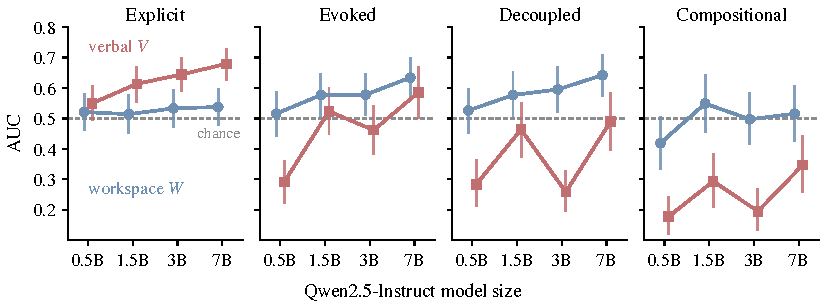
\includegraphics[width=\textwidth]{figures/fig2_regime_map.pdf}
\caption{AUC of the workspace readout ($\Wrr$), the verbal report ($\Vrep$), and
embedding relevance across model sizes (Qwen2.5-Instruct) and provenance regimes;
error bars are 95\% item-bootstrap CIs, the gray line marks chance. The two
channels trade places as provenance shifts from explicit to inferred; on the
construct-valid Decoupled benchmark the verbal report stays at or below chance at every
size. \updated{This original regime-map visualization is retained; corrected
v3 numerical results appear in the accompanying tables.}}
\label{fig:regime}
\end{figure}

\begin{table}[tbp]
\centering
\caption{Workspace and verbal ranking by provenance regime for the checkpoints discussed in the main text. Each entry is the pooled item-level AUC of the workspace readout $W$ or the verbal report $V$ (log-space yes-versus-no score through the chat template) for recovering load-bearing candidates. The first block holds three capable-scale instruct checkpoints from other families; the second is the dense Qwen3 ladder, whose 8B row is the fourth cross-family model. All 23 checkpoints appear in Table~\ref{tab:appA1}.}
\label{tab:master}
\footnotesize
\setlength{\tabcolsep}{3.8pt}
\begin{tabular}{l*{8}{c}}
\toprule
 & \multicolumn{2}{c}{Explicit} & \multicolumn{2}{c}{Evoked} & \multicolumn{2}{c}{Decoupled} & \multicolumn{2}{c}{Compositional} \\
\cmidrule(lr){2-3}\cmidrule(lr){4-5}\cmidrule(lr){6-7}\cmidrule(lr){8-9}
Model & $W$ & $V$ & $W$ & $V$ & $W$ & $V$ & $W$ & $V$ \\
\midrule
Qwen2.5-7B-Instruct & .5376 & .6792 & .6341 & .5856 & .6423 & .4897 & .5156 & .3472 \\
OLMo-2-7B-Instruct & .4938 & .6231 & .6688 & .5398 & .6664 & .3529 & .5341 & .2944 \\
Mistral-7B-Instruct-v0.3 & .5324 & .6191 & .6687 & .5777 & .6713 & .4700 & .5962 & .3242 \\
\midrule
Qwen3-1.7B & .4818 & .5917 & .5409 & .3895 & .5607 & .1961 & .4162 & .1812 \\
Qwen3-4B & .5090 & .6496 & .5744 & .4798 & .5291 & .3967 & .5050 & .2600 \\
Qwen3-8B & .5090 & .7100 & .6204 & .4534 & .6545 & .3872 & .5466 & .2079 \\
Qwen3-14B & .5083 & .7400 & .6390 & .5219 & .6677 & .4271 & .5086 & .2163 \\
Qwen3-32B & .5084 & .7480 & .6139 & .5511 & .6919 & .4782 & .5532 & .2774 \\
\bottomrule
\end{tabular}
\end{table}


\subsection{A Provenance-Dependent Dissociation}
\label{sec:dissociation}

\updatedparagraph{Table~\ref{tab:master} gives the corrected v3 grid. Across
the four capable-scale families, Decoupled $W{-}V$ is $+0.1526$, $+0.2525$,
$+0.3135$, and $+0.2014$; every paired 95\% confidence interval excludes
zero. The provenance reversal remains: verbal reporting is strongest for
surface-explicit content, while the workspace readout is consistently higher
on silently inferred Decoupled content. The correction changes the magnitude
of several cells, especially Qwen3-8B verbal AUC ($0.4020$), but not the
qualitative conclusion.}

Table~\ref{tab:master} and Fig.~\ref{fig:regime} give the central result. On
explicit content, the verbal report is the best available signal
($\Vrep$ up to $0.6792$ at 7B; it exceeds $\Wrr$ in three of four capable
families): when importance is written on the surface, asking the model
works, and cheap heuristics work well too. The asymmetry is mechanically
natural: by the end of encoding, surface mentions are largely no longer
decodable at the readout position whether useful or not (median $\Wrr$
${\approx}0.001$ for both classes on Explicit), so the readout carries
little utility signal there, while the probe re-reads the full context and
can evaluate exactly the surface content it sees. On evoked silent bridges the ordering reverses. On the construct-valid benchmarks (Decoupled here, Compositional in
\S\ref{sec:boundary}) $\Vrep$ is $0.3529$--$0.4897$ on Decoupled and $0.2944$--$0.4119$ on Compositional, at
or below chance, with confident yes-ratings concentrated on vivid
distractors, while $\Wrr$ reads $0.6423$--$0.6713$ on Decoupled (at or near
chance on Compositional for three of four families, \S\ref{sec:boundary}); on the
answer-coupled Evoked benchmark $\Vrep$ is more variable
(above chance at 7B) yet still loses to $\Wrr$ where the contrast is significant
(Table~\ref{tab:master}). The paired Decoupled difference is significant in
all four capable-scale model families under the corrected whole-episode
bootstrap (Table~\ref{tab:crossfamily}). Across
three benchmark generators the two channels differ in kind: the workspace
readout stays within a narrow band ($0.64$--$0.67$ on the capable-scale
Decoupled cells)
while the verbal channel swings from anti-calibrated to well-calibrated with
generator and scale ($0.26$--$0.88$). The boundary variable is measurable:
annotated cue density (independently evoking context elements per episode)
predicts 7B reporter success (Spearman $\rho{=}0.25$, $p{=}4\times10^{-4}$
within the primary generator) while the workspace readout is flat in it
($\rho{=}0.10$, $p{=}0.14$; full analysis in App.~\ref{app:replications}). The model knows more than it tells, and the
telling, not the knowing, is the unstable channel: a gate can bet on the
readout. We therefore use the paired gap rather than the legacy $\Ms$ values
for the corrected headline comparison. Embedding
relevance also fails on inferred bridges
(chance on Evoked/Decoupled, $0.40$ on Compositional) and the workspace beats it decisively on Decoupled
($+0.170$ $[+0.072, +0.275]$): neither self-report nor retrieval-style relevance
sees what the model inferred.
The signal is not a surface artifact: it localizes to the context token that
licenses the inference, in mid-to-late layers, rather than uniformly across
the passage or at the concept's own mention, which never occurs
(Fig.~\ref{fig:mechanism}, App.~\ref{app:causal}). This is the readout reading
a context-specific computation, consistent with its above-chance recovery
where surface and embedding relevance are at chance (Table~\ref{tab:master})
and with the causal test of \S\ref{sec:causal}.

\updatedparagraph{The corrected dense Qwen3 ladder sharpens the scale result
without supporting a universal scaling law. On Decoupled, the gap is
$+0.2433$, $+0.0429$, $+0.2525$, $+0.3196$, and $+0.3553$ at
1.7B/4B/8B/14B/32B. The 8B--32B endpoint widening is $+0.1027$ with paired
95\% CI $[+0.0093,+0.1944]$, but the 4B exception and non-monotonic adjacent
changes rule out a simple monotone claim.}

\begin{table}[H]
\centering
\caption{Corrected Qwen3 Decoupled scale sweep. The endpoint contrast
$\Delta(W{-}V)$ from 8B to 32B is $+0.1027$ with paired 95\% CI
$[+0.0093,+0.1944]$; adjacent changes are non-monotonic.}
\label{tab:scale}
\small
\setlength{\tabcolsep}{7pt}
\begin{tabular}{lrrr}
\toprule
Model & $V$ & $W$ & $W{-}V$ \\
\midrule
\updatedrow Qwen3-1.7B & 0.3174 & 0.5607 & +0.2433$^{*}$ \\
\updatedrow Qwen3-4B & 0.4862 & 0.5291 & +0.0429 \\
\updatedrow Qwen3-8B & 0.4020 & 0.6545 & +0.2525$^{*}$ \\
\updatedrow Qwen3-14B & 0.3480 & 0.6677 & +0.3196$^{*}$ \\
\updatedrow Qwen3-32B & 0.3366 & 0.6919 & +0.3553$^{*}$ \\
\bottomrule
\end{tabular}
\vspace{2pt}
\parbox{0.94\linewidth}{\scriptsize $^{*}$Paired 95\% CI on $W{-}V$ excludes zero.}
\end{table}


\begin{figure}[H]
\centering
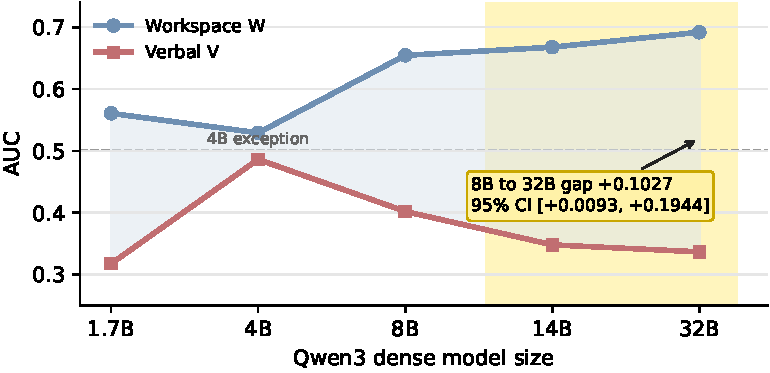
\includegraphics[width=0.82\textwidth]{figures/fig_v3_scale.pdf}
\caption{\updated{Corrected Qwen3 Decoupled scale sweep. Yellow shading marks
the newly added 14B/32B boundary region; the original figures elsewhere in
the paper are retained.}}
\label{fig:v3scale}
\end{figure}

\subsection{Limits of Static Readouts}
\label{sec:boundary}

The workspace readout does not recover every class of inferred content, and the
boundary is informative.
On Compositional, where the bridge is weakly evoked and matters only through a two-hop
composition, $\Wrr$ sits at chance for Qwen and OLMo (Mistral: $0.60$). This limitation is not an artifact of an untrained readout. Taking recovery
to mean a paired improvement over the static readout at 7B whose 95\% CI
excludes zero, a tuned future-token lens initialized at the model's own
unembedding and trained on disjoint contexts
\citep{pal2023futurelens,belrose2023tuned} does not recover Compositional
($+0.049$ $[-0.053, +0.149]$ at 7B; its only paired gain is at 0.5B, where
the absolute AUC remains near chance) and is significantly worse than the
plain logit lens on evoked bridges at 7B ($-0.088$;
App.~\ref{app:futurelens}). Across every static readout we tested, including a conditional-likelihood
score that is predictively comparable elsewhere (LL$-W$ on Compositional
$+0.078$ $[-0.040, +0.188]$, not a recovery under the paired criterion;
App.~\ref{app:vrobust}), the end-of-encoding state holds inferences that the
narrative actively evokes, rather than everything a future question might
make relevant. \S\ref{sec:extensions}
shows a gradient-based readout crosses this boundary in one of the two
families tested.

\textbf{Post-training analysis.}
In our stage sweep, none of 11 transitions improves the workspace channel:
eight Qwen base$\to$instruct pairs are flat to slightly negative, and OLMo-2's actual
pipeline declines cumulatively (base $0.631 \to$ SFT $0.599 \to$ DPO $0.576
\to$ RLVR $0.580$; $-0.052$, directional: one-sided $p{=}0.041$, two-sided
cluster CI $[-0.105, +0.007]$; App.~\ref{app:olmo}). What is unambiguous is
the absence of improvement in any of the 11 transitions. The
verbal channel's inferential-regime failure is not created by chat tuning:
raw-probed base models are erratic on inferred content (e.g., Qwen-7B
base $V_{raw}{=}0.11$ on Compositional; OLMo-2-1B base $0.445$), and the chat-tuned probe
settles at a confidently miscalibrated $0.27$--$0.30$. Post-training rewards are computed on emitted text, never on internal
availability, and the result is a fluent report channel that was never trained
against the internal one. (Scope: this concerns utility-salience; \citet{latentintrospection2026} show
that detection of injected concepts can be elicited in models, a different
construct, attributed there to in-context information rather than a
post-training mechanism.)

\begin{figure}[t]
\centering
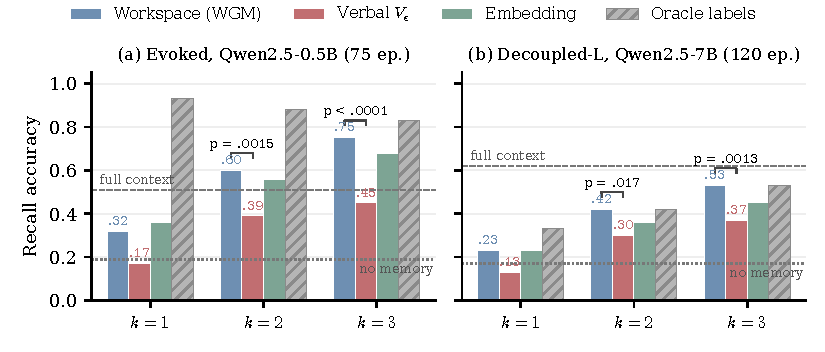
\includegraphics[width=\textwidth]{figures/fig3_downstream.pdf}
\caption{Budget-limited recall QA. Left: 0.5B on the Evoked benchmark, where
workspace gating beats verbal gating ($k{=}2$: $+20/-4$, $p{=}0.0015$; $k{=}3$: $+24/-2$,
$p{<}10^{-4}$), which sits at the no-memory floor. Right: 7B on the
construct-valid Decoupled benchmark (64-token answers), where workspace gating
matches the label oracle and beats verbal gating ($k{=}3$, $\dagger$: $+26/-7$, $p{=}0.0013$,
computed on the 120-episode scaled benchmark). The two panels are the two
regimes' primary cells; the full grid, which also contains null and reversed
cells at these $n$'s, and all McNemar tests are in
App.~\ref{app:downstream}.}
\label{fig:downstream}
\end{figure}

\subsection{Budget-Constrained Memory Selection}
\label{sec:payoff}

Fig.~\ref{fig:downstream} evaluates the two channels as write-admission policies.
At 0.5B on evoked bridges, gating on the binary importance probe stores
confidently wrong vivid words and at $k{=}1$ performs at the no-memory
floor, while workspace gating reaches $0.75$ at $k{=}3$; the paired advantage
is significant despite only 75 episodes. Budget-$k$ payoff tracks
within-episode ranking rather than the pooled AUC of Eq.~\ref{eq:auc}
(top-3 containment $0.707$ here; App.~\ref{app:downstream}). The canonical 1--10 rating variant is a
stronger verbal baseline on this answer-coupled benchmark (matching workspace
there) but sits at chance predictively on the construct-valid Decoupled benchmark
(App.~\ref{app:vrobust}).
At 7B on the $120$-episode construct-valid benchmark (Decoupled-L),
workspace gating shows no detectable
difference from the selection
oracle ($0.525$ vs.\ $0.525$ at $k{=}3$; paired difference $0.000$, 95\% CI
$[-0.092, +0.083]$; workspace nominally exceeds
the oracle in two other cells, indicating the oracle itself is noise-limited
at this $n$) and beats verbal gating on the same set
($+26/-7$, $p{=}0.0013$). Recency, random, and
the surface-feature fusion proxy lose to workspace gating throughout
(App.~\ref{app:downstream}, \ref{app:fusion}); embedding gating is the strongest
alternative but never separates from workspace downstream and is predictively
dispatched on Decoupled. Two boundary conditions: at 3B on Decoupled-class tasks the recall-time
composition step, not selection, is the binding constraint (oracle
$0.43$ vs.\ full-context $0.57$), and with a 24-token answer budget even the
oracle collapses: when the model cannot exploit a stored item at recall time,
selection quality has no effect.

\updatedparagraph{The workspace-only and oracle arms above are invariant to
the verbal-score migration. Direct comparisons that depend on the historical
Original verbal selected sets are treated as legacy evidence until their
selected sets are regenerated under v3; the new RL-QA comparison in
\S\ref{sec:newexperiments} uses a fully regenerated corrected Original arm.}

\begin{table}[t]
\centering
\caption{\textbf{Causal effect of input-side bridge steering on recall-time
answer preferences.} Real steering moves the residual stream from the
stored bridge toward a target bridge; sham uses an unrelated, norm-matched
direction. Qwen2.5 and Qwen3 checkpoints; 20 disjoint episode pairs.
A flip is a sign change in first-token target-versus-stored answer log-odds,
$\log P(a_{\rm target})-\log P(a_{\rm stored})$. Exact McNemar tests compare
paired real-versus-sham flips; exact two-sided Wilcoxon signed-rank tests
compare paired log-odds shifts. Specificity is strongest at gentle scales.}
\label{tab:causal}
\small
\begin{tabular}{llccccc}
\toprule
Model & Scale & Real flip & Sham flip & McNemar & $p$ & Wilcoxon $p$ \\
\midrule
Qwen2.5-7B & 0.5 & 0.70\dgain{+0.65} & 0.05 & $+13/-0$ & 0.0002 & 4.8e-05 \\
Qwen2.5-7B & 1.0 & 0.90\dgain{+0.60} & 0.30 & $+12/-0$ & 0.0005 & 1.9e-06 \\
Qwen2.5-3B & 0.5 & 0.60\dgain{+0.50} & 0.10 & $+11/-1$ & 0.0063 & 1.3e-04 \\
Qwen2.5-3B & 1.0 & 0.85\dgain{+0.50} & 0.35 & $+10/-0$ & 0.0020 & 3.8e-06 \\
Qwen2.5-0.5B & 1.0 & 0.75\dgain{+0.55} & 0.20 & $+11/-0$ & 0.0010 & 1.7e-04 \\
Qwen3-8B & 0.5 & 0.90\dgain{+0.75} & 0.15 & $+15/-0$ & 0.0001 & 1.9e-06 \\
Qwen3-8B & 1.0 & 0.95\dgain{+0.60} & 0.35 & $+12/-0$ & 0.0005 & 5.7e-06 \\
\bottomrule
\end{tabular}
\end{table}


\subsection{Causal Analysis}
\label{sec:causal}

The predictive results alone do not establish that the answer computation uses
the representations the readout measures; this section shows that it does.
To test this directly, we steer the residual stream along the stored bridge's
input-side difference-of-means direction \citep{zou2023repe} toward a
different bridge while the model answers from memory, versus sham directions
built from unrelated bridges on held-out episodes (20 disjoint pairs;
Fig.~\ref{fig:causal}).
Table~\ref{tab:causal}: at the gentlest scale the real direction flips the
answer in $0.60$ of pairs versus $0.10$ for sham at 3B (McNemar $+11/-1$,
$p{=}0.0063$) and in $0.70$ versus $0.05$ at 7B ($+13/-0$,
$p{=}2.4\times10^{-4}$), directionally consistent at 0.5B (tested at scale $1.0$). A flip means the
answer log-odds between the stored and the steered-toward bridge change
sign; sham directions are built from unrelated bridges of held-out episodes
at matched norm. At stronger steering scales real flips rise further but
sham flips rise too (App.~\ref{app:causal}), so the gentle-scale contrast
carries the specificity claim. Output-side (unembedding) steering has no effect, consistent with
\citet{anthropic2026workspace}. The concept representations the readout scores are therefore causally used
by memory-based answering; steering the unembedding rows (the output side)
does nothing, so the readout taps content, not output preparation.

\subsection{Gating Evaluation}
\label{sec:prgresults}

\begin{table}[t]
\centering
\caption{Write-admission policies on the mixed-provenance pool
(Explicit $\cup$ Evoked $\cup$ Decoupled-L; 283 episodes; per-benchmark
generation budgets fixed across policies; all cells from a single run
generation). Bold: column best among content-scoring policies; the two internal signals
(likelihood, workspace) are statistically indistinguishable in every cell
(all $p{\ge}0.10$) and each beats the binary probe. The absence heuristic
exploits the single-planted-inference construction and collapses on
multi-absent pools (three-act analysis, App.~\ref{app:prg}); pairwise tests
and the 1--10 rating analysis are also there.}
\label{tab:prg}
\small
\begin{tabular}{lcccc}
\toprule
\multirow{2}{*}{Policy} & \multicolumn{2}{c}{0.5B} & \multicolumn{2}{c}{7B} \\
\cmidrule(lr){2-3} \cmidrule(lr){4-5}
 & $k{=}2$ & $k{=}3$ & $k{=}2$ & $k{=}3$ \\
\midrule
Verbal (binary probe) & 0.290 & 0.329 & 0.463 & 0.555 \\
Verbal (1--10 rating) & 0.343 & 0.410 & 0.491 & 0.601 \\
Embedding & 0.350 & 0.442 & 0.477 & 0.583 \\
Cond.\ likelihood (one pass/cand.) & \textbf{0.375} & \textbf{0.466} & \textbf{0.537} & 0.618 \\
\wsrow Workspace (zero passes) & 0.332 & 0.431 & 0.502 & \textbf{0.636} \\
PRG (routed) & 0.336 & 0.417 & \textbf{0.512} & 0.565 \\
\addlinespace
\refrow Absence heuristic (diagnostic) & 0.459 & 0.459 & 0.629 & 0.636 \\
\refrow Oracle & 0.512 & 0.484 & 0.657 & 0.707 \\
\bottomrule
\end{tabular}
\end{table}

Table~\ref{tab:prg} evaluates the gate in the deployment-realistic setting: a
pooled stream mixing all three provenance regimes, where any channel that
fails on one regime pays for it. Because the contribution is an admission
score rather than a memory system, the comparison holds the pipeline fixed
and varies only the score; an end-to-end comparison against full memory
frameworks would confound retrieval, organization, and prompting with the
admission signal under study, and every such framework can adopt whichever
score wins here. Three results follow.

\myparagraph{The workspace gate beats the binary probe.}
Replacing the
binary importance probe with the workspace readout wins at $k{=}3$ at both
scales ($+47/-18$, $p{=}0.0004$, confirmatory under Holm correction over the
full test family; $+45/-22$, $p{=}0.0067$ uncorrected, marginal after
correction; App.~\ref{app:prg}),
and the workspace channel is never significantly worse than any
content-scoring policy in any cell.

\myparagraph{The failure is specific to the verbal channel, not to internal signals generally.}
Against the canonical 1--10
rating, the strongest verbal form, workspace gating is numerically ahead at
7B ($0.636$ vs.\ $0.601$, $p{=}0.31$) at zero probe cost, where the rating
spends one forward pass per candidate, and on the construct-valid slice the
rating is predictively at or below chance (App.~\ref{app:vrobust}). An
internal conditional-likelihood score at that same one-pass cost gates
indistinguishably from the workspace readout (all cells $p{\ge}0.10$) and
itself beats the binary probe ($p{\le}0.035$ in three of four cells,
$p{=}0.051$ in the fourth; App.~\ref{app:prg}); the readout is the internal
signal that needs no extra passes and carries the causal grounding of
\S\ref{sec:causal}.

\myparagraph{At tight budgets, provenance routing adds a little more.}
At the tight 7B budget provenance routing is the strongest policy
that spends no per-candidate forward passes ($0.512$ vs.\ $0.502$
single-channel) and helps where the channels are complementary; the single-channel
gate is the recommended default at capable scale. Calibration matters:
$z$-normalized routing loses admission slots for inferred items
systematically because the two score distributions differ in shape, and
underperforms rank calibration throughout (App.~\ref{app:prg}). Finally,
because each benchmark plants a single inference, bare absence is nearly an
oracle proxy here; App.~\ref{app:prg} analyzes this diagnostic and the
multi-absent stress tests, where the degenerate absence heuristic collapses
and, when the competing absent candidates are semantically confusable, the
workspace readout is the leading channel: its selection-signal advantage
over the embedding replicates on a fresh 120-episode set (paired
$\Delta$AUC $+0.064$, one-sided $p{=}0.026$; pooled estimate $+0.058$
$[+0.007, +0.108]$) and gated QA shows no
detectable difference from the true-label oracle (App.~\ref{app:prg}).
On the two standard naturalistic streams (LoCoMo, LongMemEval), whose
candidates are surface content by construction, no question-blind channel,
ours or the verbal importance probe, separates from random under LLM-judge
grading:
the construct that separates the channels is structurally absent there, which
is precisely why the controlled benchmarks of \S\ref{sec:benchmarks} are
needed. When that construct is planted back, by embedding our Decoupled
episodes inside real LoCoMo sessions, the dissociation reappears at 7B with
the workspace readout unattenuated ($W{-}V$ $+0.21$ $[+0.10, +0.31]$): the
effect is carried by content provenance, not by synthetic style
(App.~\ref{app:locomo}).

\section{Metacognitive Alignment and Availability Readouts}
\label{sec:extensions}

\begin{table}[t]
\centering
\caption{\textbf{Metacognitive alignment}, two model families: ${\sim}$500
fine-tuning steps on yes/no labels derived from each model's own workspace
ranking, using disjoint benchmarks (Evoked, Explicit, Evoked-G2). The verbal
channel is repaired on fully held-out benchmarks (+0.28--0.39 AUC) while the
workspace channel is untouched, full-context QA is statistically unchanged,
and general capability (MMLU, GSM8K, ARC) is unaffected (Table~\ref{tab:geneval})
(App.~\ref{app:metacog}). For the Qwen-0.5B Compositional row the repaired
reporter converges to its teacher's (chance) level; where generation-time
computation adds signal (OLMo Compositional) the student can exceed the
static teacher (\S\ref{sec:metacog}).}
\label{tab:metacog}
\small
\resizebox{\textwidth}{!}{%
\begin{tabular}{llcccc}
\toprule
\multirow{2}{*}{Model} & \multirow{2}{*}{Held-out benchmark} & \multicolumn{2}{c}{Verbal report $V$ (AUC)} & \multicolumn{2}{c}{Workspace $W$} \\
\cmidrule(lr){3-4} \cmidrule(lr){5-6}
 & & before & after & before & after \\
\midrule
OLMo-2-1B & Decoupled & 0.326 [0.251, 0.400] & \textbf{0.671}\dgain{+0.35} [0.584, 0.751] & 0.580 & 0.586 \\
OLMo-2-1B & Compositional & 0.267 [0.179, 0.360] & \textbf{0.580}\dgain{+0.31} [0.482, 0.677] & 0.477 & 0.491 \\
\addlinespace
Qwen2.5-0.5B & Decoupled & 0.281 [0.210, 0.354] & \textbf{0.668}\dgain{+0.39} [0.595, 0.737] & 0.526 & 0.524 \\
Qwen2.5-0.5B & Compositional & 0.172 [0.112, 0.241] & \textbf{0.451}\dgain{+0.28} [0.367, 0.534] & 0.416 & 0.409 \\
\bottomrule
\end{tabular}
}
\end{table}


\begin{figure}[t]
\centering
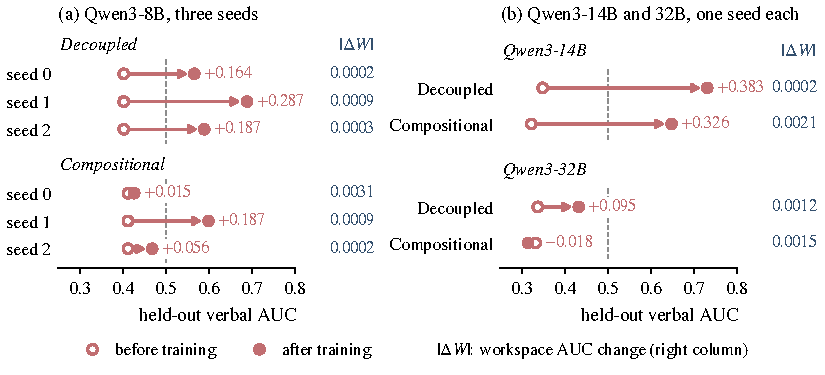
\includegraphics[width=0.95\textwidth]{figures/fig4_development_repair.pdf}
\caption{\textbf{Post-training changes the verbal channel, not the workspace
channel, and the verbal channel is repairable.} \textbf{(a)}~OLMo-2-1B released post-training stages: the
workspace channel ($W$, blue) never improves from base, on either benchmark, while
the verbal channel ($V$, rose) stays at chance (Evoked) or far below it
(Compositional). \textbf{(b)}~Metacognitive alignment: ${\sim}500$ self-distillation
steps move the verbal channel (arrows) from below-chance to well-calibrated on fully
held-out benchmarks while leaving the workspace channel in place (open circle =
before, filled = after).}
\label{fig:devrepair}
\end{figure}

\subsection{Metacognitive Alignment}
\label{sec:metacog}

If the model knows more than it tells because telling was never trained
against the knowing (Fig.~\ref{fig:devrepair}), the reporter should be
trainable from the model's own workspace signal, without human annotation. We fine-tune OLMo-2-1B-Instruct for ${\sim}500$ steps on
the exact importance-probe prompt, with yes/no targets derived from the model's
own workspace ranking (top-2 items per episode), using only the explicit and
evoked benchmarks plus the second-generator benchmark (Evoked-G2, gpt-4o); the decoupled benchmarks
(Decoupled, Compositional) are never seen. Table~\ref{tab:metacog} (seed-0 runs; three-seed means $0.62$--$0.65$,
App.~\ref{app:metacog}): held-out verbal calibration jumps from $0.326$ to
$0.671$ and from $0.267$ to $0.580$. The same procedure,
unchanged, replicates in a second family: Qwen2.5-0.5B-Instruct rises from
$0.281$ to $0.668$ (Decoupled) and $0.172$ to $0.451$ (Compositional).
Three controls secure the interpretation: label-shuffled fine-tunes leave
held-out calibration at chance in both families ($0.416$/$0.382$),
distilling from embedding-derived labels fails ($0.458$), and the aligned
reporter rejects context-absent foils ($0.900$), so the gain is specifically
the workspace signal, not format de-biasing, generic salience, or an absence
shortcut (App.~\ref{app:metacog}). The two Compositional endpoints then fit one
prediction: distillation transfers the monitor's signal, so where the static
teacher is at chance (Qwen-0.5B) the student plateaus there, while where
generation-time computation adds signal beyond the static snapshot (OLMo-1B)
the student can exceed the static value, behaving like the dynamic readouts
of \S\ref{sec:family}. The calibration
transfers across held-out benchmarks and generators, which is consistent with the
reporter acquiring a benchmark-independent readout of internal state; shared
construction biases across generators cannot be fully excluded. The workspace channel itself is untouched, and
full-context QA never moves significantly ($-0.029$ for OLMo, $+0/-2$,
$p{=}0.50$; $-0.044$ for Qwen, $+5/-8$, $p{=}0.58$; App.~\ref{app:metacog}). Practically, twenty minutes of self-supervised fine-tuning on one GPU repairs
a channel that SFT, DPO, and RLVR left miscalibrated.

\subsection{A Family of Availability Readouts}
\label{sec:family}

\begin{table}[t]
\centering
\caption{Availability readouts by provenance regime, Qwen-7B AUC.
Full grids and confidence intervals are in App.~\ref{app:family}.
The paired Compositional contrast is $W_J{-}W$: $+0.125$
[$+0.010$, $+0.244$]; App.~\ref{app:vrobust} gives the
conditional-likelihood comparison. Bold marks the column best.}
\label{tab:family}
\small
\begin{tabular}{lccc}
\toprule
Member & Evoked & Decoupled & Compositional \\
\midrule
Spotlight $W$ (static) & 0.633 & \textcolor{gain}{\textbf{0.641}} & 0.514 \\
Broadcast breadth (static) & 0.637 & 0.557 & 0.486 \\
Rehearsal $W_{rep}$ (dynamic) & \textcolor{gain}{\textbf{0.684}} & 0.578 & 0.553 \\
Leverage $W_{J}$ (dynamic) & 0.506 & 0.550 & \textcolor{gain}{\textbf{0.639}} \\
\bottomrule
\end{tabular}
\end{table}


Availability to downstream computation can be operationalized in more than one
way. We evaluate four readouts of the same frozen model: \emph{Spotlight}
($\Wrr$, instantaneous decodability), \emph{Broadcast} (its spatial spread across
positions, in the spirit of global-workspace ignition, \citealp{dehaene2011}),
\emph{Rehearsal} ($W_{rep}$: reactivation across $K$ sampled probe-blind
continuations, an analogue of offline replay), and Leverage ($W_J$: the
directional
derivative of expected future answering utility along the concept's input-side
direction, the infinitesimal form of the causal intervention in
\S\ref{sec:causal}, computed by backpropagation without training: one
forward-plus-backward pass per episode--question pair, with every candidate
scored from the same gradient). The expectation $\mathbb{E}_q$ is over a fixed
bank of 12 probe-blind questions per episode, scored on the model's own greedy
answers $\hat a_q$.
Table~\ref{tab:family} shows a clean double dissociation between readouts:
decode-based members own the evoked regime (Rehearsal reaches $0.684$ on Evoked,
improving on Spotlight), while Leverage is the only member that recovers
compositional bridges under the paired criterion of \S\ref{sec:boundary}
(Compositional at 7B: $0.639$; paired over Spotlight $+0.125$
$[+0.010, +0.244]$, CI excluding zero), at the cost of low sensitivity where decoding is easy. Rehearsal's Compositional
ceiling ($\approx 0.55$) does not move with rollout budget: free-running
generation rarely performs the composition spontaneously, whereas the gradient
detects the latent structure without requiring it to run. Boundaries: the Leverage result does not
replicate on OLMo-2-7B ($0.515$); head-to-head against the
conditional-likelihood baseline on Compositional the two do not separate
($W_J{-}$LL $+0.046$ $[-0.056, +0.153]$, App.~\ref{app:vrobust}), so the
claim is that Leverage is the only \emph{workspace} readout whose paired
gain over the static member is significant, not that it beats every
non-workspace score; and naive member ensembles do not beat the
per-regime best member (App.~\ref{app:family}); availability estimation is regime- and family-dependent, and the dissociation
between readouts parallels, at a lower level, the report--computation
dissociation that motivates this work.

\section{New Experimental Evidence}
\label{sec:newexperiments}

\updatedparagraph{This section adds the experiments collected after the
original manuscript. It preserves the paper's original thesis---workspace
availability is a better admission signal for silently inferred content---and
tests how far that thesis survives corrected measurement, larger scale, and
two distinct repair mechanisms.}

\subsection{Corrected cross-family measurement}

\begin{table}[tbp]
\centering
\caption{Workspace--report comparison on Decoupled across four model families. $W$: workspace readout; $V$: yes/no importance report from Eq.~\eqref{eq:score}. Intervals for $W{-}V$ are paired 95\% whole-episode bootstrap intervals from 4,000 draws.}
\label{tab:crossfamily}
\small
\setlength{\tabcolsep}{4.5pt}
\begin{tabular}{lrrrr}
\toprule
Model & $V$ & $W$ & $W{-}V$ & 95\% CI \\
\midrule
Qwen2.5-7B-Instruct & 0.4897 & 0.6423 & \textbf{+0.1526} & [+0.0500, +0.2582] \\
Qwen3-8B & 0.3872 & 0.6545 & \textbf{+0.2673} & [+0.1670, +0.3668] \\
OLMo-2-7B-Instruct & 0.3529 & 0.6664 & \textbf{+0.3135} & [+0.2297, +0.3992] \\
Mistral-7B-Instruct-v0.3 & 0.4700 & 0.6713 & \textbf{+0.2014} & [+0.1000, +0.3015] \\
\bottomrule
\end{tabular}
\end{table}


\updatedparagraph{The v3 log-space score preserves the central dissociation
at capable scale. Qwen2.5-7B-Instruct, Qwen3-8B, OLMo-2-7B-Instruct, and
Mistral-7B-Instruct all have positive Decoupled workspace--report gaps, and
all four paired confidence intervals exclude zero. The smallest gap is
$+0.1526$ and the largest is $+0.3135$. This is the corrected quantitative
version of the original cross-family claim; the mechanism and causal results
do not consume $V$ and therefore do not change under the migration.}

\subsection{Workspace-derived supervision at 8B and beyond}

\begin{table}[H]
\centering
\caption{Binary Metacognitive Alignment under the corrected verbal score.
Qwen3-8B is the three-seed primary result; 14B/32B are single-seed exploratory
boundary measurements. Yellow marks newly added or re-measured rows.}
\label{tab:alignment}
\scriptsize
\setlength{\tabcolsep}{3.2pt}
\resizebox{\textwidth}{!}{%
\begin{tabular}{llrrrrrl}
\toprule
Model & Seed & $V_{\rm before}$ & $V_{\rm after}$ & $\Delta V$ & $\Delta W$ & Comp. $\Delta V$ & Verdict \\
\midrule
\updatedrow Qwen3-8B & 0 & 0.4020 & 0.5662 & \textbf{+0.1642} & +0.00017 & +0.0145 & GREEN \\
\updatedrow Qwen3-8B & 1 & 0.4020 & 0.6889 & \textbf{+0.2868} & +0.00091 & +0.1873 & Strong GREEN \\
\updatedrow Qwen3-8B & 2 & 0.4020 & 0.5893 & \textbf{+0.1873} & -0.00028 & +0.0564 & GREEN \\
\addlinespace
\updatedrow Qwen3-14B & 0 & 0.3480 & 0.7306 & \textbf{+0.3826} & -0.00017 & +0.3261 & Strong GREEN \\
\updatedrow Qwen3-32B & 0 & 0.3366 & 0.4320 & \textbf{+0.0954} & +0.00116 & -0.0176 & AMBER \\
\bottomrule
\end{tabular}}
\end{table}


\updatedparagraph{Binary Metacognitive Alignment now has a three-seed
capable-scale replication. Every Qwen3-8B seed clears the preregistered
Decoupled $\Delta V\ge 0.15$ gate, with mean $+0.2128$ and sample standard
deviation $0.0652$. Workspace AUC changes by less than $0.001$ and
full-context QA changes by at most $1.47$ points, so this is a reporter repair
rather than a change in the teacher or general answering behavior. Transfer
is narrower: Compositional mean $\Delta V$ is $+0.0861$, with only seed 1
clearing the same gate. The 14B and 32B rows are single-seed boundary probes;
the 14B peak is strong, while 32B is directional but AMBER, so the evidence
does not support monotonic repair scaling.}

\subsection{Probe-blind learning of memory action}

\begin{table}[H]
\centering
\caption{Probe-blind RL-QA on Decoupled at budget two. Admission is evaluated
against the corrected Original verbal policy; recall uses the frozen,
adapter-disabled checkpoint.}
\label{tab:rlqa}
\scriptsize
\setlength{\tabcolsep}{3pt}
\resizebox{\textwidth}{!}{%
\begin{tabular}{llrrrrll}
\toprule
Model & Seed & Original QA & RL-QA QA & $\Delta$QA & $\Delta$ admission AUC & 95\% CI & Verdict \\
\midrule
\updatedrow Qwen3-8B & 0 & 1.47\% & 8.82\% & \textbf{+7.35 pp} & \textbf{+0.4339} & [+0.3743,+0.5022] & PASS \\
\updatedrow Qwen3-8B & 1 & 1.47\% & 7.35\% & \textbf{+5.88 pp} & \textbf{+0.4216} & [+0.3645,+0.4855] & PASS \\
\updatedrow Qwen3-8B & 2 & 1.47\% & 10.29\% & \textbf{+8.82 pp} & \textbf{+0.4599} & [+0.4086,+0.5203] & PASS \\
\addlinespace
\updatedrow Qwen3-32B & 0 & 7.35\% & 11.76\% & \textbf{+4.41 pp} & \textbf{+0.3653} & [+0.3056,+0.4423] & unresolved \\
\bottomrule
\end{tabular}}
\end{table}


\updatedparagraph{RL-QA never observes the workspace readout or the verbal
importance probe. It learns a budget-2 admission policy from downstream QA
reward and is evaluated with the adapter disabled during recall. Across three
Qwen3-8B seeds, admission AUC improves by $+0.4216$--$+0.4599$ and recall by
$+5.88$--$+8.82$ points over the regenerated v3 Original policy. Absolute
recall remains low, so this closes the admission loop rather than solving
long-horizon recall. At 32B, admission improves by $+0.3653$, but QA gains only
$+4.41$ points and misses the preregistered $+5$-point gate; this is an
admission-positive, QA-unresolved boundary result.}

\subsection{One diagnosis, two repair targets}

\updatedparagraph{The additions strengthen the original story without
changing its subject. The workspace signal still diagnoses the gap and
supports the training-free gate. Workspace-derived self-distillation repairs
what the model \emph{says} should be remembered. Probe-blind RL-QA separately
repairs what the agent \emph{does} store. Only the first repair consumes
workspace-derived supervision; keeping the two paths separate avoids claiming
that all successful memory decisions must explicitly read the workspace.}

\section{Conclusion}
\label{sec:conclusion}

An importance report's ordering follows its candidate pool's provenance
structure. SDA turns internal rankings into admission supervision and
exceeds each model's own report in all 54 comparisons on the
statedness-balanced pool. Standard serving preserves recall.
Memory systems can train admission before the future question
arrives and retain the inferred links that answering will need.


\bibliographystyle{iclr2027_conference}
\bibliography{references}

\clearpage
\appendix
\section{Benchmark Construction and Leakage Audit}
\label{app:benchmarks}

\subsection{Passages, concepts and future questions}

The primary author model is GPT-4.1. Each episode contains a passage,
candidate concepts with construction-assigned utility labels, and a
future question and answer. Explicit places useful content in the
passage. \textbf{Implied-answer} training episodes cue an unstated
useful concept that itself supplies the answer, including episodes from
the alternate-author benchmark. The extended tables use this name for
that training construction. Decoupled requires an unstated bridge to support a further
inference: the answer is absent from the passage and candidate set,
and the question shares no passage content word except a protagonist's
name. Compositional requires a multi-hop inference and permits question
anchors from the passage. Decoupled and Compositional are development
batteries used for configuration selection and excluded from gradient
training.

Mechanical validation checks candidate strings, bridge absence, answer
exclusion and the Decoupled question's lexical overlap. Concept
deduplication removes repeated concepts across retained episodes.
The leakage audit additionally checks full lexemes, inflected answers
and question anchors. A blind GPT-6-Astra alias audit receives the
future question, gold answer and bridge. It rejects identity,
morphological or derivational variants, synonyms, translations,
abbreviations and containment that trivially yields the answer.
For example, \emph{caterer/catering} is an alias, whereas
\emph{Madrid/Spanish} requires a further inference. The audit records
the verdict and exclusion reason for each episode.

\subsection{Episode-authoring prompt}
\label{app:authorprompt}
GPT-4.1 receives the system instruction, ``You are a careful dataset
designer for a cognitive-science experiment on LLM memory.'' The
following prose transcription preserves the generation constraints;
the output-format instruction requests one structured record per episode.
\begin{sdabox}{Episode-authoring prompt}
Design a batch of diverse test episodes about silent bridge reasoning
for a memory experiment. Each episode has a passage of four to eight
sentences about a named person; invent a distinctive first name,
different in every episode, and vary the domain widely. A question
asked later, out of context, refers to the episode only through the
person's name and requires an unstated bridge fact inferable from the
passage, followed by common general knowledge. Supply a short correct
answer of one to three words and five to seven candidate concepts,
each a common lowercase word with a utility category and a short reason.

Exactly one candidate is the useful bridge concept, and its word must
be absent from the passage. The question must share no passage content
word except the person's name: someone who never read the passage
must be unable to answer it. For a passage about Elena wandering the
Plaza Mayor, ask what language Elena should have brushed up on for her
trip, without naming the plaza in the question. The answer must differ
from every candidate and be absent from the passage; combining the
bridge with general knowledge yields the answer. For example, the
Plaza Mayor cues \emph{madrid}, which supports \emph{spanish}. A reader
remembering only the bridge plus the question must be able to answer.

Include two or three vivid, emotional or surprising distractors that
occur literally in the passage but are useless for the question, and
one or two neutral concepts that occur in the passage. Every candidate
must be a single common English lowercase word. Do not reuse concepts
or person names across episodes.
\end{sdabox}
Generation uses temperature 1.0 and batches of up to five episodes.
Mechanical filters and the alias audit apply after generation.

\subsection{Frozen batteries and replication benchmarks}
\label{app:fresh}

Fresh-1 and Fresh-2 use the Decoupled construction prompt and mechanical
filters, followed by deduplication and disjointness filtering. A context
match after lowercasing and trimming against a prior battery causes
exclusion. A bridge matching a construction-labeled training concept
also causes exclusion. Fresh-2 additionally excludes contexts appearing
in Fresh-1. Shared answer categories, such as languages and currencies,
are permitted. The retained batteries contain 316 and 363 episodes,
respectively. The alternate-author benchmark repeats the inferred-concept
construction with a different author model. The entity-bridge benchmark
places a named-entity bridge among scene-object distractors.

\subsection{Reconstructing the reported controls}
\label{app:pools}
\label{app:controls}

All pool interventions traverse the 363 held-out Fresh-2 episodes in
their frozen order and preserve the question, answer and original
utility labels. Added candidates receive negative utility labels.
Within an episode, original candidates precede additions, whose recorded
order is retained. The frozen control archive records the passages,
ordered additions, named candidates and context permutation; replay uses
these recorded draws. The standard pool contains 1,607 candidates,
4.43 per episode. Statedness uses the case-insensitive stem match
specified in \S\ref{sec:setup}.

\paragraph{A worked source episode.}
The first episode reads: ``Yara compared renewal quotes from different
insurers online and reviewed her accident history. She called the hotline
to ask clarifying questions about premium increases. After considering
the coverage limits and deductibles, Yara finally entered her payment
details to confirm the policy.'' Its candidates, in order, are
\emph{insurer, deductible, history, policy, insurance}; \emph{insurance}
is useful. The question is ``Which professional would be most relevant
for Yara to contact regarding her recent purchase?'' and the answer is
\emph{agent}. The second episode is Jibril's visit in
Figure~\ref{fig:episode}.

\paragraph{Stated-bridge, position and distractor-named controls.}
The exact sentence form is ``The passage also mentions \emph{concept}.''
The stated-bridge control appends this sentence with the useful concept;
the position control prepends it. The distractor-named control appends
it with the first non-useful candidate in the original order. Thus
Yara's stated-bridge control adds ``The passage also mentions insurance.''
after the passage, the position control puts that sentence before
``Yara compared,'' and the distractor-named control instead appends
``The passage also mentions insurer.'' These three controls keep all
five candidates and their order unchanged.

\paragraph{Pool with unstated distractors.}
An author model proposes four single-word concepts from the useful
concept's semantic category, asking for alternatives a careless reader
might confuse with it but that the passage does not imply. The instruction
requires lowercase words absent from the passage and a comma-separated
response. We retain the response order, discard a proposal that matches
an original candidate or occurs as a case-insensitive substring of the
passage, and append the accepted concepts. The frozen pool contains
1,450 additions: four in 361 episodes and three in episodes 24 and 263
after filtering, giving 3,057 candidates in total (8.42 per episode).
For Yara, the ordered additions are \emph{warranty, mortgage, pension,
annuity}; her passage and five original candidates stay fixed.
The development confusable-distractor control applies the same procedure
to Decoupled. The unrelated-distractor control instead takes bridges
from subsequent episodes, as described for the enlarged pool below.

\paragraph{Statedness-balanced pool.}
Odd positions, counting from one, keep the original passage; even
positions append ``The passage also mentions \emph{concept}.'' with
the useful concept substituted. Every episode keeps its original
candidates and takes the first four accepted additions at odd positions
or the first three at even positions from the pool with unstated
distractors, preserving their order. This yields 2,877 candidates,
7.93 per episode. Yara occupies position one, so her passage is unchanged
and her pool is the five original candidates followed by \emph{warranty,
mortgage, pension, annuity}. Jibril occupies position two: append
``The passage also mentions dubai.'' to Figure~\ref{fig:episode}'s
passage and append \emph{doha, riyadh, muscat} to its six candidates.
The original question and answer remain fixed in each case.

\paragraph{Naming-balanced pool.}
\label{app:namingpool}
Use the same ordered candidate lists as the statedness-balanced pool,
but start from the original passages. Name four candidates per episode.
At odd positions exclude the useful concept and sample four other
candidates uniformly without replacement; at even positions include the
useful concept and sample three others. Use one Python standard
pseudorandom generator seeded with zero, process episodes in frozen
order, prepend the useful concept to the sampled list when included,
and shuffle each selected list before constructing sentences. Sampling
and shuffling consume the same continuing random stream. The five
sentence forms, in rotation, are ``The passage also mentions
\emph{concept}.'', ``\emph{concept} is relevant here.'', ``Note that
\emph{concept} comes up as well.'', ``There is also \emph{concept} to
consider.'', and ``\emph{concept} features in this as well.''

Number episodes and insertions from zero for the placement rule. The
first selected candidate uses the sentence form at the episode's
position in the five-form cycle; each subsequent candidate advances
one form. Strip trailing full stops from the original passage, split
at full-stop--space boundaries, trim each segment and restore one full
stop to each. Before each insertion, count the current sentence list,
including earlier additions. The insertion boundary is the remainder
of the episode index plus three times the insertion index upon division
by that count plus one. Boundary zero precedes the passage; the final
boundary follows it. Insertions thus advance through an evolving
sentence list rather than all occurring at its end.

For Yara, the shuffled selection is \emph{pension, annuity, insurer,
policy}. The additions are ``The passage also mentions pension.'',
``annuity is relevant here.'', ``Note that insurer comes up as well.'',
and ``There is also policy to consider.'' Their successive insertion
boundaries are zero, three, zero and two. The final passage begins with
the insurer, pension and policy sentences, then Yara's first two original
sentences, then the annuity sentence, then her final original sentence.
There are 1,452 naming interventions, 181 of which name the useful
concept: a named candidate is useful 12.5\% of the time, against the
12.6\% base rate among 2,877 candidates. Questions, answers and
candidate order stay fixed.

\paragraph{Enlarged pool.}
Combine the standard candidate list, the accepted same-topic additions,
and four bridges from other episodes. To choose the latter, start with
the next episode in frozen order, advance cyclically, and accept a bridge
only if it is absent from the passage, absent from the original
candidate list and distinct from earlier accepted bridges. Stop after
four accepted bridges. Concatenate the three lists in this order and
retain the first occurrence of each concept. The resulting 4,506
candidates average 12.41 per episode. Yara's pool is \emph{insurer,
deductible, history, policy, insurance, warranty, mortgage, pension,
annuity, dubai, church, kanji, doctor}. Her passage, question and answer
remain unchanged. The unrelated-distractor control uses just the
standard candidates and the four cross-episode additions; for Yara
these are \emph{dubai, church, kanji, doctor}.

\paragraph{Shuffled context and bridge replacement.}
Shuffled context uses the archived episode permutation, replacing each
passage while preserving its own candidates, utility labels, question
and answer. The first episode receives the passage at position 105,
about Lars skating on slick tracks with thin-bladed boots; its candidates
remain Yara's five concepts and its answer remains \emph{agent}.
The bridge-replacement control acts on SDA's recorded top-two selections
only when they contain the useful concept: retain the other selection
and replace the useful concept with the next-ranked candidate, then
replay the same frozen reader and question. For a selection of
\emph{dubai, elevator} with \emph{gift} next, the replayed memory is
\emph{gift, elevator}; Jibril's question and \emph{arabic} answer stay
fixed. This example illustrates the replacement rule; the measured
249 replays use the recorded selections (\S\ref{app:episodemetrics}).

\paragraph{Candidate proposal and reader references.}
The context-only proposer receives the original passage and the
instruction in Appendix~\ref{app:prompts}; the future question and bridge
are hidden. Its parsed output replaces the supplied candidate list in
proposal order. For Yara the resulting candidates are \emph{online,
accident, hotline, premium, coverage, deductibles, payment, policy},
so \emph{insurance} is unavailable to admission. At two stored concepts,
the same frozen reader answers from each policy's selected pair.
The question-only reference gives that reader Yara's question with no
memory; the whole-passage reference gives the same question and her
original three-sentence passage. Neither reference performs admission.
The wording controls change only the admission instruction, whose five
exact forms appear in Appendix~\ref{app:wording}. Authorship and
entity-bridge controls repeat the episode construction with the authors
and concept categories specified in Appendix~\ref{app:replications}.

SDA improves ranking and retention under the naming-balanced construction
(Table~\ref{tab:namingbalanced}). Across Qwen3-8B seeds, within-episode
AUC is 0.715--0.725, versus 0.566 for the report and 0.636 for the
workspace readout. Useful-concept retention at $k=2$ is 53.2--54.0\%,
versus 24.0\% and 40.8\%, respectively.

\begin{table}[htbp]
\centering
\caption{Naming-balanced pool recall across 363 episodes. Every episode names four candidates using five sentence templates; a named candidate is useful at the base rate. Recall is reported in percent under blind semantic grading at one, two and three stored concepts for six models. Report is the model's own yes/no importance report; Rating is the 1--10 importance rating \citep{park2023generative}; SDA is the mean of three seeds.}
\label{tab:namingrecall}
\small
\setlength{\tabcolsep}{3.5pt}
\begin{tabular}{lccccccccc}
\toprule
& \multicolumn{3}{c}{$k=1$} & \multicolumn{3}{c}{$k=2$} & \multicolumn{3}{c}{$k=3$} \\
\cmidrule(lr){2-4} \cmidrule(lr){5-7} \cmidrule(lr){8-10}
Model & Report & Rating & \textbf{SDA} & Report & Rating & \textbf{SDA} & Report & Rating & \textbf{SDA} \\
\midrule
Qwen3-8B & 27.6 & 35.3 & \textbf{36.4} & 42.7 & 45.2 & \textbf{46.2} & 46.3 & 47.1 & \textbf{47.0} \\
Qwen3-14B & 21.8 & 30.3 & \textbf{33.7} & 33.3 & 36.4 & \textbf{40.8} & 41.3 & 43.2 & \textbf{41.2} \\
Qwen3-32B & 31.7 & 30.0 & \textbf{41.1} & 43.2 & 43.0 & \textbf{48.9} & 50.7 & 51.8 & \textbf{53.4} \\
Qwen2.5-7B & 9.4 & 11.6 & \textbf{13.3} & 21.2 & 25.6 & \textbf{28.3} & 28.6 & 33.3 & \textbf{33.0} \\
OLMo-2-7B & 24.8 & 30.6 & \textbf{37.0} & 39.4 & 43.0 & \textbf{46.7} & 44.6 & 52.1 & \textbf{49.5} \\
Mistral-7B & 4.7 & 5.8 & \textbf{9.9} & 9.6 & 13.2 & \textbf{16.0} & 19.8 & 21.5 & \textbf{23.7} \\
\bottomrule
\end{tabular}
\end{table}

\begin{table}[htbp]
\centering
\caption{Candidate ranking and useful-concept retention on the naming-balanced pool, Qwen3-8B, 363 episodes and 2,877 candidates. Every episode names four candidates using five sentence templates at varying positions. A named candidate is useful 12.5\% of the time, against a 12.6\% base rate. AUC uses construction utility labels; retention is in percent.}
\label{tab:namingbalanced}
\small
\setlength{\tabcolsep}{4pt}
\begin{tabular}{lccccc}
\toprule
Admission policy & \shortstack{Pooled\\AUC} & \shortstack{Episode\\AUC} & $B_1$ & $B_2$ & $B_3$ \\
\midrule
Yes/no importance report & 0.570 & 0.566 & 9.4 & 24.0 & 42.7 \\
Workspace readout & 0.635 & 0.636 & 22.0 & 40.8 & 54.8 \\
\textbf{SDA, seed 0} & \textbf{0.726} & \textbf{0.725} & \textbf{36.1} & \textbf{54.0} & \textbf{67.5} \\
\textbf{SDA, seed 1} & \textbf{0.714} & \textbf{0.715} & \textbf{32.2} & \textbf{54.0} & \textbf{65.6} \\
\textbf{SDA, seed 2} & \textbf{0.728} & \textbf{0.725} & \textbf{35.5} & \textbf{53.2} & \textbf{68.0} \\
\bottomrule
\end{tabular}
\end{table}


\section{SDA Training and Scoring Details}
\label{app:training}

\subsection{Teacher construction and data split}

Within each episode, let $r_S(c)$ be a candidate's ascending mid-rank
under readout $S$, with ties assigned the average of their occupied
ranks. For $m>1$ candidates, the percentile is
\begin{equation}
P_S(c;x)=\frac{r_S(c)-1}{m-1},
\qquad S\in\{W,\mathrm{LL}\}.
\label{eq:percentile}
\end{equation}
For a singleton pool the percentile is one half. Averaging the
percentiles yields the teacher in Eq.~\eqref{eq:teacher}; descending
teacher score and then candidate order determine the top-2 labels.
Both frozen readouts score the same episode and candidate before these
labels are constructed.

A source group is one author-and-construction battery: Explicit
(88 episodes), implied-answer from the primary author (75), or
implied-answer from the alternate author (57). The split is stratified
by these groups and assigns whole episodes, including all their candidates,
to training or validation. Within each group, episodes are sorted by a
cryptographic hash of the fixed split seed and the source-qualified
episode identity; the lowest 20\%, rounded up, enter validation.
The split seed is zero and stays fixed across optimization seeds.
This gives 70/18, 60/15 and 45/12 training/validation episodes in the
three groups, respectively: 175 training and 45 validation episodes in total. The teacher generates every
optimization target from these passages and candidates.
The selection protocol is specified in \S\ref{sec:student}.

\subsection{Complete training configuration}
\label{app:configuration}

LoRA adapts the attention query, key, value and output projections and
the feed-forward gate, up and down projections. Base parameters remain
frozen. Each model supplies its own teacher rankings and receives its
own admission adapter. The two highest-ranked candidates in each
training episode receive positive admission targets; all remaining
candidates receive negative targets. Only the target word contributes
to the vocabulary-normalized cross-entropy in Eq.~\eqref{eq:loss}.
Prompt tokens are masked. Qwen3 uses its chat template with thinking
disabled.

\begin{center}
\small
\begin{tabular}{@{}p{0.30\linewidth}p{0.64\linewidth}@{}}
\toprule
Setting & Configuration \\
\midrule
Adapter & Low-rank adaptation, rank 16, scaling 32; attention and
feed-forward projections \\
Optimizer & AdamW; constant learning rate $1\times10^{-5}$ \\
Batching & Batch size 1; gradient accumulation over 4 batches \\
Training duration & Two epochs; 414 optimizer steps \\
Sequence length & At most 1024 tokens \\
Data & 175 training and 45 validation episodes; source-stratified, disjoint episodes \\
Targets & Two highest teacher ranks positive; all others negative \\
\bottomrule
\end{tabular}
\end{center}

\subsection{Measurement conventions}
\label{app:conventions}

The yes/no report in every main table is scored in log space over the
yes and no token sets. The wording comparison uses its own common
scorer for all five wordings, so its rows are comparable to one another
under that aggregation: Mistral-7B's passage-only wording gives AUC
0.411 in the main tables and 0.440 in the wording comparison because
the two scorers aggregate differently; scoring the same wording one
prompt at a time also gives 0.440, identical to the batched result.
On Qwen3-8B's standard pool, first-token workspace AUC is 0.543 at
the end of the passage and 0.530 when the candidate is appended and
the state is read immediately before its first token; the latter is
the matched baseline for full-candidate AUC 0.574.
Frozen-report recall is 40.8\% in the main tables and 40.5\% in the
objective ablation, which evaluates the untrained checkpoint through
the adapter-loading path instead of the frozen path.

\subsection{Admission baselines}
\label{app:baselines}

SDA is compared with the following baselines. The \textbf{yes/no
importance report} uses the untrained model's score $V$ in
Eq.~\eqref{eq:score}, with Qwen3 thinking disabled.
The \textbf{1--10 importance rating} is the expected rating under
normalized probabilities of the complete answer strings.
The \textbf{reversed yes/no report} admits the lowest-scoring candidates.
\textbf{Admit what the passage omits} prioritizes candidates absent from
the passage under the statedness test and breaks ties at random.
\textbf{Omission then report} prioritizes unstated candidates and
uses the yes/no importance report to order candidates within each
provenance. The \textbf{provenance-adjusted report} adds a single
coefficient times the candidate's statedness indicator to the untrained
report, with the coefficient fitted on development episodes and held
fixed for evaluation. The \textbf{combined teacher used directly} ranks
by Eq.~\eqref{eq:teacher} without training an adapter.
The \textbf{implied-content wording} permits implied
content; the \textbf{provenance-cued wording} explicitly says the
passage may never mention the useful concept (App.~\ref{app:wording}).
\textbf{Random selection} samples candidates uniformly; \textbf{output
likelihood} and the \textbf{workspace readout} rank candidates directly
by their respective scores. Each baseline sees the passage and candidates
with the future question hidden. \textbf{Oracle labels} prioritize the
intended bridge; question-only and whole-passage readers provide recall
references. Bold entries identify SDA throughout the comparison tables.

\subsection{Exact admission, reader, rating and proposal instructions}
\label{app:prompts}

The boxes below reproduce the natural-language instructions. Italic
phrases stand for the supplied passage, candidate, memory list or
question. Each is a user message rendered with the model's chat template
and assistant generation prefix; Qwen3 thinking is disabled. SDA and the
report baseline share the admission prompt.

\begin{sdabox}{Admission prompt}
\emph{Passage}

Based only on the passage above, is the concept ``\emph{candidate
concept}'' one of the most important things to remember in order to
answer possible future questions? Answer with a single word: yes or no.
\end{sdabox}
The affirmative token set contains the distinct first tokens of
\emph{yes} in lowercase, initial-capital and uppercase forms, with
and without a leading space. The negative set is constructed analogously
from \emph{no}. Equation~\eqref{eq:score} gives the common report
score; SDA applies the same scoring rule with its adapter enabled.

\begin{sdabox}{Reader prompt}
Earlier you read a passage. The only things you remember from it are:
\emph{stored concepts separated by commas}.\\
Using only what you remember, answer concisely.\\
Question: \emph{future question}\\
Answer:
\end{sdabox}
The reader uses the frozen model with its admission adapter disabled.
The question-only reference asks ``Answer this question concisely.''
followed by the question and answer prefix. The whole-passage reference
supplies the passage, then ``Answer concisely.'' and the same question
and answer prefix. Greedy decoding is used throughout.

\begin{sdabox}{Rating baseline prompt}
\emph{Passage}

On a scale of 1 to 10, where 1 is purely mundane and 10 is extremely
important, rate how important it is to remember the concept
``\emph{candidate concept}'' in order to answer possible future questions
about this passage. Answer with a single number.
\end{sdabox}
Let $a_r$ be the complete answer string for rating $r$, and let $u_R(c,x)$
be this prompt. Each answer receives its full sequence probability,
multiplying the conditional probabilities of its tokens. The score is
\begin{equation}
\begin{split}
R(c;x)&=\sum_{r=1}^{10}r\,\pi_r(c;x),\\
\pi_r(c;x)&=\frac{p_{\mathcal M}(a_r\mid u_R(c,x))}
{\sum_{j=1}^{10}p_{\mathcal M}(a_j\mid u_R(c,x))}.
\end{split}
\label{eq:rating}
\end{equation}
A rating represented by multiple tokens is scored as a complete answer.

\begin{sdabox}{Candidate-proposal prompt}
\emph{Passage}

A memory system can store only a few single-word concepts about the
passage above. List up to 8 concepts that could be worth remembering
for possible future questions, including things the passage clearly
implies but does not state. Answer with lowercase single words separated
by commas, and nothing else.
\end{sdabox}
The context-only proposer uses Qwen3-8B with greedy decoding. Distinct
parsed concepts form the candidate pool. The bridge, future question
and answer are withheld from proposal and carried forward for evaluation.
Bridge coverage accepts case differences and a trailing plural ending.

\subsection{Ablation protocol}
\label{app:ablationprotocol}

The teacher and optimization ablations in \S\ref{sec:ablations} use the
same training episodes, adapter shape and matched step budget. The
recall-reward condition samples admitted sets from the admission scores
and asks the frozen reader to answer from the selected memory. Answer
correctness supplies the reward. Within each rollout group, reward
differences are normalized into advantages; updates use a clipped
group-relative policy objective and a penalty for departure from the
frozen policy \citep{shao2024deepseekmath}. The future question enters
the reward computation. The refinement condition applies these updates
after SDA training.

\section{Documented Prospective Freeze}
\label{app:freeze}

The dated experiment record documents prospective freezes of Fresh-1
and Fresh-2 on 15 September 2026. It records each battery's episode
count and cryptographic digest before evaluated models read it: 316
episodes for Fresh-1 and 363 for Fresh-2. The accompanying reproducibility
record retains the dated entries and verified battery digests.
Fresh-1 supplied the initial frozen-battery evaluation.
Fresh-2 was frozen before any evaluated model read it
and after configuration selection. Its primary endpoint compares SDA
with the yes/no report; a primary training seed was designated and the
remaining seeds reported alongside it. Its secondary endpoint compares
SDA with the rating baseline. Fresh confirmation uses the blind semantic
judge in App.~\ref{app:judge}.

\section{Recall Grading and Serving Protocol}
\label{app:repro}

\subsection{Blind semantic judge}
\label{app:judge}

The judge, GPT-6-Astra, receives the question, gold answer and reader
response with no admission-policy identity. The substantive grading
instruction is quoted verbatim; its output-format instruction requests
a label for every supplied answer.
\begin{sdabox}{Grading instruction}
Grade short answers to memory questions. For each item decide whether
ANSWER gives GOLD as its answer.\\
Labels:\\
``correct'': the answer commits to GOLD or an exact equivalent (synonym,
inflection, fuller name) as its single answer. Extra explanation is fine.\\
``hedged'': it offers two or more alternative answers (e.g.\ ``X or Y''),
or states the answer cannot be determined, even if GOLD is mentioned.\\
``incorrect'': anything else, including a different answer.
\end{sdabox}
Only correct responses contribute to recall; hedged and incorrect
responses count as errors. Judgments are reused for identical question,
gold answer and response triples. The harness additionally grades each
answer by string matching after normalization. Agreement is 85.1\%
across 13,068 answers; every training run exceeds its own report under
both graders, with maximum exact McNemar $p=0.026$.

\subsection{Amortized scoring time and throughput}
\label{app:timing}

The timing evaluation loads Qwen3-8B on one A100-80GB and constructs an
admission prompt for each of the 1,607 standard-pool Fresh-2 candidates. vLLM enables
prefix caching and LoRA serving, warms the engine on an initial subset,
and times batched generation over the full candidate list. Each prompt
generates one token greedily; SDA attaches the adapter to the admission
request, while the report baseline uses the same engine without it.
Model loading is outside the timed region. Milliseconds per candidate
are wall time divided by candidate count; throughput is candidate count
divided by wall time. The served and reference selections are passed
to the same frozen reader and semantic judge. The serving engine
recovers yes/no masses from returned token log probabilities.

\subsection{Capability with the adapter enabled on every token}
\label{app:capability}

Enabling the adapter on every token changes the four measured capability
scores by at most 0.3 percentage points under matched prompts.
Base and adapter scores are
71.6\% and 71.5\% on MMLU \citep{hendrycks2021mmlu}, 80.4\% and
80.7\% on ARC-Easy, 56.2\% and 56.4\% on ARC-Challenge
\citep{clark2018arc}, and 88.4\% and 88.6\% on the GSM8K evaluation
subset \citep{cobbe2021gsm8k}. The deployed interface attaches the
adapter to admission requests.


\section{Recall across Evaluation Batteries and Pools}
\label{app:recall}

SDA exceeds the report in all 54 comparisons across six
models, three seeds and three budgets. All seeds reach exact McNemar
$p<0.05$ in 17 of 18 model--budget cells; Qwen3-32B at $k=3$ has
maximum $p=0.073$. Across the six models, pooled report AUC is
0.658--0.736 and workspace AUC is 0.719--0.812.


\begin{table}[htbp]
\centering
\caption{Paired SDA minus baseline recall differences on the statedness-balanced pool, Qwen3-8B, for every row of Table~\ref{tab:balancedbaselines}, which cites each published method (1--10 importance rating \citep{park2023generative}; ConsistencyGate \citep{consistencygate2026}; A-MAC \citep{amac2026}; prediction error \citep{nemori2026}). Entries average three seeds and give 95\% intervals from 4,000 paired bootstrap draws over 363 episodes. Differences are in percentage points.}
\label{tab:balancedpaired}
\footnotesize
\setlength{\tabcolsep}{3pt}
\begin{tabular}{lccc}
\toprule
Baseline & $k=1$ & $k=2$ & $k=3$ \\
\midrule
\multicolumn{4}{l}{\emph{Importance judgments of the untrained model}} \\
Yes/no importance report & $+9.9$ [$+6.1$, $+13.8$] & $+10.7$ [$+7.0$, $+14.6$] & $+6.3$ [$+2.9$, $+9.7$] \\
1--10 importance rating & $+4.7$ [$+1.0$, $+8.3$] & $+5.2$ [$+1.7$, $+8.8$] & $+1.1$ [$-2.4$, $+4.6$] \\
Implied-content wording & $+9.1$ [$+5.4$, $+12.9$] & $+9.1$ [$+5.7$, $+12.7$] & $+4.1$ [$+1.0$, $+7.3$] \\
\addlinespace
\multicolumn{4}{l}{\emph{Admission criteria from published methods}} \\
ConsistencyGate, sampled & $+16.5$ [$+11.6$, $+21.5$] & $+18.7$ [$+14.1$, $+23.6$] & $+11.0$ [$+6.3$, $+15.5$] \\
ConsistencyGate, single pass & $+16.0$ [$+10.8$, $+21.1$] & $+18.7$ [$+14.0$, $+23.5$] & $+9.4$ [$+4.8$, $+14.1$] \\
A-MAC utility & $+10.5$ [$+5.6$, $+15.3$] & $+14.1$ [$+9.3$, $+19.0$] & $+6.9$ [$+2.6$, $+11.1$] \\
Prediction error & $+24.0$ [$+18.9$, $+29.1$] & $+27.8$ [$+22.5$, $+33.2$] & $+21.5$ [$+16.4$, $+26.6$] \\
\addlinespace
\multicolumn{4}{l}{\emph{Provenance rules}} \\
Provenance-adjusted report & $+3.9$ [$-0.9$, $+8.5$] & $+14.6$ [$+9.5$, $+19.8$] & $+11.8$ [$+6.4$, $+17.0$] \\
Reversed yes/no report & $+16.8$ [$+11.5$, $+22.2$] & $+24.0$ [$+18.5$, $+29.5$] & $+18.7$ [$+13.2$, $+24.3$] \\
Admit what the passage omits & $+11.8$ [$+6.4$, $+17.3$] & $+21.8$ [$+16.3$, $+27.2$] & $+15.4$ [$+10.0$, $+21.1$] \\
Omission then report & $+3.6$ [$-1.0$, $+8.6$] & $+14.6$ [$+9.4$, $+19.7$] & $+11.8$ [$+6.5$, $+17.2$] \\
\addlinespace
\multicolumn{4}{l}{\emph{Internal signals used directly}} \\
Output likelihood used directly & $+5.8$ [$+0.6$, $+10.7$] & $+11.8$ [$+6.7$, $+16.9$] & $+10.2$ [$+5.3$, $+15.1$] \\
Combined teacher used directly & $+3.6$ [$-1.2$, $+8.2$] & $+8.8$ [$+3.9$, $+13.9$] & $+5.5$ [$+0.9$, $+10.0$] \\
\bottomrule
\end{tabular}
\end{table}


Qwen3-8B SDA improves mean recall over the report on each development
and frozen battery in Table~\ref{tab:sdamain}. The gains also occur
with unstated distractors and in the enlarged pool
(Tables~\ref{tab:stress} and~\ref{tab:bigpool}). Across all six models,
mean SDA recall exceeds the report and rating at every standard-pool
budget (Tables~\ref{tab:sdabudget} and~\ref{tab:baselines}).

\begin{table*}[t]
\centering
\caption{Recall accuracy (\%) at $k{=}2$ on Qwen3-8B, blind semantic grading.
Development batteries (left); two frozen fresh Decoupled batteries
(right). SDA: mean\,$\pm$\,SD over three seeds. $^{*}$every seed
exceeds the yes/no report with exact McNemar $p<0.05$. Rating: 1--10
importance rating \citep{park2023generative}.}
\label{tab:sdamain}
\small
\setlength{\tabcolsep}{3pt}
\begin{tabular}{lcccccc}
\toprule
 & \multicolumn{4}{c}{Development} & \multicolumn{2}{c}{Fresh (held out)} \\
\cmidrule(lr){2-5} \cmidrule(lr){6-7}
Admission policy & Decoupled & Compositional & Confusable & Unrelated & Fresh-1 & Fresh-2 \\
 & $n{=}68$ & $n{=}52$ & $n{=}68$ & $n{=}68$ & $n{=}316$ & $n{=}363$ \\
\midrule
Yes/no importance report & 35.3 & 46.2 & 35.3 & 36.8 & 34.8 & 40.8 \\
1--10 importance rating & 47.1 & 53.8 & 48.5 & 48.5 & 43.7 & 45.7 \\
\wsrow \textbf{SDA} & \textbf{49.5}\,$\pm$\,2.2 & \textbf{54.5}\,$\pm$\,1.1 & \textbf{48.5}\,$\pm$\,2.5 & \textbf{50.0}\,$\pm$\,2.5 & \textbf{44.2}\,$\pm$\,0.7$^{*}$ & \textbf{50.0}\,$\pm$\,1.4$^{*}$ \\
\addlinespace
\refrow Oracle labels & 51.5 & 65.4 & 51.5 & 51.5 & 50.0 & 54.3 \\
\bottomrule
\end{tabular}
\end{table*}


\begin{table}[tbp]
\centering
\caption{Recall on the pool with unstated distractors (Fresh-2 with four extra candidates per episode that the passage also never states, 8.4 candidates per episode). Blind semantic grading, recall in percent, three training seeds per model; $p$ bounds the exact McNemar test against each model's own yes/no report across those seeds.}
\label{tab:stress}
\small
\setlength{\tabcolsep}{4pt}
\begin{tabular}{lcccc}
\toprule
Model & Yes/no report & \textbf{SDA (3 seeds)} & $p$ vs.\ report & Oracle labels \\
\midrule
Qwen3-8B & 41.0 & \textbf{51.0 / 51.2 / 49.9} & $\leq$ $10^{-3}$ & 54.3 \\
Qwen3-14B & 32.2 & \textbf{40.8 / 39.4 / 39.9} & $\leq$ $10^{-3}$ & 46.6 \\
Qwen3-32B & 41.0 & \textbf{51.0 / 50.7 / 50.1} & $\leq$ $10^{-4}$ & 54.8 \\
Qwen2.5-7B & 23.7 & \textbf{31.4 / 28.4 / 30.6} & $\leq$ .019 & 31.7 \\
OLMo-2-7B & 38.8 & \textbf{52.3 / 51.0 / 51.2} & $\leq$ $10^{-5}$ & 54.8 \\
Mistral-7B & 12.9 & \textbf{19.0 / 19.6 / 17.9} & $\leq$ .015 & 16.8 \\
\bottomrule
\end{tabular}

\end{table}

\begin{table}[tbp]
\centering
\caption{Recall on the enlarged pool: Fresh-2 with 12.41 candidates per episode, up from 4.43. Qwen3-8B, blind semantic grading, recall in percent. Output likelihood is used directly. SDA entries give three training seeds; $p$ bounds the exact McNemar test against the report across seeds. Oracle labels prioritize the intended bridge.}
\label{tab:bigpool}
\small
\setlength{\tabcolsep}{3pt}
\begin{tabular}{lcccccc}
\toprule
Budget & \shortstack{Yes/no\\report} & \shortstack{Output\\likelihood} & \shortstack{Workspace\\readout} & \textbf{SDA (3 seeds)} & $p$ vs.\ report & \shortstack{Oracle\\labels} \\
\midrule
$k=1$ & 29.5 & 28.1 & 24.0 & \textbf{38.0 / 38.0 / 39.7} & $\leq$ $10^{-4}$ & 47.1 \\
$k=2$ & 40.5 & 32.0 & 34.7 & \textbf{50.7 / 52.6 / 51.2} & $\leq$ $10^{-5}$ & 54.3 \\
$k=3$ & 41.9 & 33.9 & 38.6 & \textbf{52.9 / 52.1 / 52.1} & $\leq$ $10^{-5}$ & 51.5 \\
\bottomrule
\end{tabular}

\end{table}


\begin{table}[t]
\centering
\caption{Memory budget across models. Recall accuracy (\%) on the held-out Fresh-2 battery (363 episodes) with $k$ stored concepts; each model admits memories with its own adapter and answers with its own frozen weights; blind semantic grading; Rating is the 1--10 importance rating \citep{park2023generative}; SDA is the mean over three seeds; $^{*}$every seed exceeds the yes/no report of the same model at that budget (exact McNemar $p<0.05$).}
\label{tab:sdabudget}
\small
\setlength{\tabcolsep}{4pt}
\begin{tabular}{lccccccccc}
\toprule
 & \multicolumn{3}{c}{$k{=}1$} & \multicolumn{3}{c}{$k{=}2$} & \multicolumn{3}{c}{$k{=}3$} \\
\cmidrule(lr){2-4} \cmidrule(lr){5-7} \cmidrule(lr){8-10}
Model & Report & Rating & \textbf{SDA} & Report & Rating & \textbf{SDA} & Report & Rating & \textbf{SDA} \\
\midrule
Qwen3-8B & 28.1 & 34.7 & \textbf{37.6}$^{*}$ & 40.8 & 45.7 & \textbf{50.0}$^{*}$ & 41.6 & 47.9 & \textbf{52.2}$^{*}$ \\
Qwen3-14B & 23.4 & 31.1 & \textbf{33.5}$^{*}$ & 32.5 & 39.1 & \textbf{40.5}$^{*}$ & 37.5 & 43.5 & \textbf{43.6}$^{*}$ \\
Qwen3-32B & 32.5 & 32.0 & \textbf{41.4}$^{*}$ & 41.0 & 44.6 & \textbf{50.2}$^{*}$ & 46.0 & 50.7 & \textbf{53.0}$^{*}$ \\
Qwen2.5-7B-Instruct & 9.6 & 9.6 & \textbf{16.8}$^{*}$ & 23.1 & 22.6 & \textbf{29.8}$^{*}$ & 29.5 & 35.0 & \textbf{35.8}$^{*}$ \\
OLMo-2-7B-Instruct & 27.5 & 33.1 & \textbf{48.5}$^{*}$ & 38.0 & 44.1 & \textbf{55.4}$^{*}$ & 44.4 & 52.6 & \textbf{56.9}$^{*}$ \\
Mistral-7B-Instruct & 5.2 & 9.6 & \textbf{12.4}$^{*}$ & 12.7 & 15.7 & \textbf{19.8}$^{*}$ & 19.3 & 22.0 & \textbf{24.2}$^{*}$ \\
\bottomrule
\end{tabular}
\end{table}


\begin{table*}[t]
\centering
\caption{Admission policies on Qwen3-8B: standard pool and pool with unstated
distractors. Blind semantic grading, recall in percent. Output
likelihood is used directly. Rows above the rule are untrained
baselines; dashes denote unmeasured settings.}
\label{tab:baselines}
\small
\setlength{\tabcolsep}{4pt}
\begin{tabular}{lcccccc}
\toprule
 & \multicolumn{3}{c}{Standard pool} & \multicolumn{3}{c}{\shortstack{Pool with unstated\\distractors}} \\
\cmidrule(lr){2-4}\cmidrule(lr){5-7}
Admission policy & $k=1$ & $k=2$ & $k=3$ & $k=1$ & $k=2$ & $k=3$ \\
\midrule
Yes/no importance report & 28.1 & 40.8 & 41.6 & 28.6 & 41.0 & 41.3 \\
1--10 importance rating \citep{park2023generative} & 34.7 & 45.7 & 47.9 & 35.8 & 46.6 & 48.8 \\
Reversed yes/no report & 35.5 & 46.6 & 49.0 & 23.4 & 28.9 & 30.9 \\
Admit what the passage omits & 46.6 & 53.4 & 49.6 & 31.7 & 35.3 & 36.9 \\
Random selection & 28.6 & 44.6 & 46.6 & --- & --- & --- \\
Output likelihood & --- & 48.8 & --- & 30.6 & 39.1 & 40.5 \\
Workspace readout & 29.8 & 44.6 & 49.9 & 26.7 & 39.4 & 44.9 \\
\midrule
\textbf{SDA (mean of 3 seeds)} & \textbf{37.6} & \textbf{50.0} & \textbf{52.2} & \textbf{37.6} & \textbf{50.7} & \textbf{51.6} \\
\addlinespace
\refrow Oracle labels & 47.1 & 54.3 & 51.5 & 47.1 & 54.3 & 51.5 \\
\bottomrule
\end{tabular}

\end{table*}


\begin{table*}[t]
\centering
\caption{Paired SDA--baseline recall differences on three candidate pools,
Qwen3-8B. Entries are seed-averaged differences in points with 95\%
intervals from 4,000 paired bootstrap draws over episodes.
All comparisons use the same frozen reader and blind semantic judge.}
\label{tab:paired}
\small
\setlength{\tabcolsep}{3pt}
\begin{tabular}{lccc}
\toprule
Baseline & $k=1$ & $k=2$ & $k=3$ \\
\midrule
\multicolumn{4}{l}{\emph{Standard pool}} \\
\quad Yes/no importance report & $+9.6$ [$+5.8$, $+13.3$] & $+9.3$ [$+5.2$, $+13.2$] & $+10.6$ [$+6.8$, $+14.1$] \\
\quad 1--10 importance rating & $+2.9$ [$-0.6$, $+6.4$] & $+4.3$ [$+0.9$, $+7.8$] & $+4.2$ [$+1.3$, $+7.2$] \\
\quad Provenance-cued wording & $+5.4$ [$+1.4$, $+9.4$] & $+7.1$ [$+2.9$, $+11.4$] & $+6.2$ [$+2.8$, $+9.7$] \\
\quad Reversed yes/no report & $+2.1$ [$-3.3$, $+7.4$] & $+3.5$ [$-1.9$, $+8.9$] & $+3.1$ [$-1.3$, $+7.5$] \\
\quad Admit what the passage omits & $-8.9$ [$-13.1$, $-4.6$] & $-3.4$ [$-7.7$, $+1.0$] & $+2.6$ [$-1.2$, $+6.2$] \\
\quad Omission then report & $-9.5$ [$-13.7$, $-5.3$] & $-3.4$ [$-7.0$, $+0.4$] & $-0.5$ [$-3.2$, $+2.4$] \\
\quad Random selection & $+9.0$ [$+4.1$, $+14.1$] & $+5.4$ [$+0.6$, $+10.3$] & $+5.6$ [$+1.4$, $+9.8$] \\
\addlinespace
\multicolumn{4}{l}{\emph{Pool with unstated distractors}} \\
\quad Yes/no importance report & $+8.9$ [$+5.1$, $+12.8$] & $+9.6$ [$+5.5$, $+13.8$] & $+10.3$ [$+6.3$, $+14.1$] \\
\quad 1--10 importance rating & $+1.7$ [$-1.6$, $+5.0$] & $+4.1$ [$+0.6$, $+7.6$] & $+2.9$ [$-0.4$, $+6.2$] \\
\quad Reversed yes/no report & $+14.1$ [$+9.0$, $+19.5$] & $+21.8$ [$+16.2$, $+27.6$] & $+20.8$ [$+15.3$, $+26.1$] \\
\quad Admit what the passage omits & $+5.9$ [$+0.6$, $+10.9$] & $+15.4$ [$+10.3$, $+20.8$] & $+14.7$ [$+9.6$, $+19.8$] \\
\quad Omission then report & $-8.4$ [$-12.7$, $-4.2$] & $+5.8$ [$+0.8$, $+10.8$] & $+8.9$ [$+4.0$, $+13.8$] \\
\quad Output likelihood & $+7.0$ [$+1.7$, $+12.0$] & $+11.6$ [$+6.5$, $+16.8$] & $+11.1$ [$+6.2$, $+16.1$] \\
\addlinespace
\multicolumn{4}{l}{\emph{Enlarged pool}} \\
\quad Yes/no importance report & $+9.1$ [$+5.2$, $+12.9$] & $+11.0$ [$+6.7$, $+15.2$] & $+10.5$ [$+6.6$, $+14.2$] \\
\quad 1--10 importance rating & $+2.2$ [$-1.3$, $+5.6$] & $+4.7$ [$+0.9$, $+8.4$] & $+4.1$ [$+0.9$, $+7.6$] \\
\quad Omission then report & $-5.5$ [$-9.6$, $-1.5$] & $+6.6$ [$+1.6$, $+11.6$] & $+12.1$ [$+7.1$, $+17.2$] \\
\quad Output likelihood & $+10.5$ [$+5.0$, $+15.7$] & $+19.6$ [$+14.3$, $+24.9$] & $+18.5$ [$+13.3$, $+23.6$] \\
\quad Random selection & $+17.1$ [$+12.4$, $+22.0$] & $+24.5$ [$+19.1$, $+29.9$] & $+22.6$ [$+17.4$, $+27.7$] \\
\bottomrule
\end{tabular}

\end{table*}


\subsection{Candidate-pool comparisons}
\label{app:poolresults}

\paragraph{The standard pool rewards omission.}
The useful concept is the only candidate the passage never states in
95\% of standard-pool episodes. The omission baseline therefore reaches 46.6\%,
53.4\% and 49.6\% recall at $k=1,2,3$, respectively; omission then
report reaches 47.1\%, 53.4\% and 52.6\%, and the reversed
report reaches 35.5\%, 46.6\% and 49.0\%. SDA's corresponding means
are 37.6\%, 50.0\% and 52.2\%. The omission cue identifies the useful
concept directly in these episodes.

\paragraph{Unstated distractors separate useful admission from omission.}
The pool with unstated distractors adds four unstated distractors per episode.
Under blind semantic grading, SDA exceeds each model's own yes/no
report in 54 of 54 comparisons across six models, three seeds and
budgets $k=1,2,3$. All three
seeds reach exact McNemar $p<0.05$ in 17 of 18 model--budget cells;
the exception is Mistral-7B at $k=3$. At $k=2$, the largest $p$ across
models and seeds is 0.019 (Table~\ref{tab:stress}).
On Qwen3-8B, direct output likelihood reaches 30.6/39.1/40.5\%
recall at $k=1,2,3$, against SDA's 37.6/50.7/51.6\% means.
SDA leads the measured non-oracle baselines at $k=2,3$;
omission then report leads at $k=1$
(Tables~\ref{tab:baselines} and~\ref{tab:paired}). At $k=2$, the omission baseline falls from
53.4\% to 35.3\% and the reversed report from 46.6\% to 28.9\%, both
below the report's 41.0\%; SDA reaches 51.0\%, 51.2\% and
49.9\%. Every SDA seed exceeds the omission baseline
at every budget, with exact McNemar $p\leq0.097$ at $k=1$ and
$p\leq6.5\times10^{-7}$ at $k=2,3$; every seed exceeds the reversed
report with $p\leq4.3\times10^{-7}$ across budgets. SDA recalls are
37.7\% / 36.4\% / 38.6\% at $k=1$ and 51.8\% / 51.5\% / 51.5\%
at $k=3$; the rating baseline reaches 35.8\% and 48.8\%.

\paragraph{Naming the bridge and changing its category test reversal.}
On the stated-bridge control at $k=2$, SDA reaches 55.4\%, 55.6\% and
52.9\% recall, against 44.9\% for the report and 39.9\% for the
reversed report. On the entity-bridge benchmark, the reversed report
reaches 0.281 admission AUC, while SDA reaches 0.987, 0.980 and 0.987,
with within-episode AUC 1.000. The direction required by reversal is a
property of candidate construction, and is opposite on this benchmark
(\S\ref{sec:gap}).

\paragraph{The enlarged pool preserves gains at two and three concepts.}
With 12.41 candidates per episode, SDA reaches 38.0\% / 38.0\% / 39.7\%
at $k=1$, 50.7\% / 52.6\% / 51.2\% at $k=2$, and
52.9\% / 52.1\% / 52.1\% at $k=3$ (Table~\ref{tab:bigpool}).
The rating baseline reaches 36.4\%, 46.8\% and 48.2\%, respectively;
every SDA seed leads it at every budget. The paired mean differences
are $+2.2$ points ($[-1.3,+5.6]$), $+4.7$ ($[+0.9,+8.4]$), and
$+4.1$ ($[+0.9,+7.6]$), respectively (Table~\ref{tab:paired}).
Omission then report has the highest recall at $k=1$; SDA leads the
measured non-oracle baselines at $k=2,3$. Direct output likelihood reaches
28.1/32.0/33.9\%, against SDA's 38.6/51.5/52.4\% means.
Random selection reaches 21.5\%, 27.0\% and
29.8\%, the report 29.5\%, 40.5\% and 41.9\%, and the workspace
readout 24.0\%, 34.7\% and 38.6\%.


\subsection{Within-episode ranking and bridge retention}
\label{app:episodemetrics}

SDA improves both within-episode ranking and retention of the intended
bridge at $k=2$ (Table~\ref{tab:episodemetrics}). Paired whole-episode
bootstrap intervals compare each score with the report baseline.
Conditional recall distinguishes retaining the bridge from answering
the question: for the primary SDA seed, recall is 54.6\% with the
bridge and 41.2\% without it, versus 48.2\% and 37.7\% for the report.

The paired replacement experiment replays the primary SDA seed's
two selections. On the 249 episodes whose memory contains the bridge,
we replace only that concept with SDA's next-ranked candidate, keeping
the other selection, question and frozen reader fixed. Recall changes
from 54.6\% to 37.8\%, a 16.9-point decrease: 59 previously correct
answers become incorrect and 17 become correct (exact McNemar
$p=1.4\times10^{-6}$). Retaining the bridge supplies information
used by the reader.

\begin{table}[tbp]
\centering
\caption{Within-episode admission ranking on the standard Fresh-2 pool (Qwen3-8B). AUC and its difference from the report have paired 95\% whole-episode bootstrap intervals (4,000 draws). Retention is the percentage of episodes whose two admitted concepts contain the useful concept.}
\label{tab:episodemetrics}
\small
\setlength{\tabcolsep}{4pt}
\begin{tabular}{lccc}
\toprule
Admission score & \shortstack{Per-episode AUC\\{}[95\% CI]} & \shortstack{$\Delta$ vs.\ report\\{}[95\% CI]} & \shortstack{Bridge retained\\($k=2$)} \\
\midrule
Yes/no report & 0.326 [0.286, 0.366] & \emph{reference} & 29.8 \\
1--10 rating \citep{park2023generative} & 0.608 [0.567, 0.648] & $+0.282$ [$+0.246$, $+0.320$] & 61.2 \\
Workspace readout & 0.547 [0.511, 0.584] & $+0.221$ [$+0.172$, $+0.271$] & 51.0 \\
Output likelihood & 0.619 [0.582, 0.654] & $+0.293$ [$+0.242$, $+0.344$] & 59.2 \\
\textbf{SDA (seed 0)} & \textbf{0.682} [0.641, 0.721] & $+0.356$ [$+0.320$, $+0.393$] & \textbf{68.6} \\
\textbf{SDA (seed 1)} & \textbf{0.679} [0.639, 0.718] & $+0.353$ [$+0.316$, $+0.391$] & \textbf{69.7} \\
\textbf{SDA (seed 2)} & \textbf{0.688} [0.648, 0.727] & $+0.362$ [$+0.325$, $+0.401$] & \textbf{69.2} \\
\bottomrule
\end{tabular}

\end{table}


\paragraph{Bridge labels and reader success measure different outcomes.}
Qwen3-8B recall is 22.9\% with the question alone, 63.9\% with the
whole passage, 54.3\% with oracle labels and 50.0\% with SDA.
Oracle labels prioritize the intended bridge; the reader answers from
the complete stored set and its own knowledge. On OLMo-2-7B and
Mistral-7B, SDA reaches 55.4\% and 19.8\%, versus 54.8\% and 16.8\%
for oracle labels.



\section{Provenance, Wording and Pool-Composition Measurements}
\label{app:provenance}

\subsection{Ranking among candidates with the same provenance}
\label{app:withinprovenance}

The report discriminates usefulness among unstated candidates.
Restricting the pool with unstated distractors to episodes with an
unstated useful concept and at least one unstated negative leaves
345 episodes, with 5.01 qualifying candidates per episode on average.
Within this group, report AUC is 0.880--0.897 across six models and
workspace AUC is 0.592--0.697. Every paired 95\% interval for workspace
minus report lies below zero (Table~\ref{tab:withinunstated}).
This measurement holds provenance fixed; the full-pool comparison
measures the competition between stated and unstated candidates.

\begin{table*}[t]
\centering
\caption{Useful-concept ranking restricted to unstated candidates in the pool with unstated distractors. The 345 qualifying episodes have an unstated useful concept and at least one unstated negative, averaging 5.01 candidates in the restricted set. Entries are pooled AUC; $W-V$ gives the workspace--report difference with a paired 95\% whole-episode bootstrap interval from 4,000 draws.}
\label{tab:withinunstated}
\small
\setlength{\tabcolsep}{5pt}
\begin{tabular}{lccc}
\toprule
Model & Yes/no report & Workspace readout & $W-V$ [95\% CI] \\
\midrule
Qwen3-8B & 0.881 & 0.639 & $-0.242$ [$-0.274$, $-0.211$] \\
Qwen3-14B & 0.880 & 0.654 & $-0.226$ [$-0.257$, $-0.196$] \\
Qwen3-32B & 0.896 & 0.697 & $-0.199$ [$-0.228$, $-0.170$] \\
Qwen2.5-7B & 0.897 & 0.592 & $-0.305$ [$-0.340$, $-0.270$] \\
OLMo-2-7B & 0.883 & 0.661 & $-0.221$ [$-0.252$, $-0.191$] \\
Mistral-7B & 0.880 & 0.672 & $-0.208$ [$-0.238$, $-0.178$] \\
\bottomrule
\end{tabular}
\end{table*}


\subsection{The full-pool AUC changes with the comparison pairs}
\label{app:composition}

On Fresh-2, the useful concept is stated in 5\% of episodes and
negative candidates in 99\%; in 95\% of episodes, the useful concept
is the sole candidate absent from the passage. Adding unstated
distractors leaves every original Qwen3-8B report score unchanged.
It adds 1,450 negative candidates to the original 1,244, while retaining
the same 363 positives. Useful-concept AUC against the added negatives
is 0.889, compared with 0.322 against the original negatives.
The pooled AUC is therefore the weighted average
\begin{equation}
\begin{split}
\mathrm{AUC}_{\mathrm{expanded}}
&=\frac{1244}{2694}\,\mathrm{AUC}_{\mathrm{original}}\\
&\quad+\frac{1450}{2694}\,\mathrm{AUC}_{\mathrm{added}}\\
&=0.627.
\end{split}
\label{eq:pooldecomposition}
\end{equation}
The added comparisons account for 53.8\% of all positive--negative
pairs. They raise AUC without changing the ordering of the original
candidates. At a two-concept budget, the report continues to prioritize
passage content: recall is 41.0\%, against SDA's 51.0\%, 51.2\% and
49.9\% across seeds (Table~\ref{tab:baselines}).

\subsection{Wording changes the importance ordering}
\label{app:wording}

Five matched wordings keep the episode, candidates and utility labels
fixed. They ask about passage-only importance, remove that restriction,
allow implied content (\emph{implied-content wording}), state that the
passage may omit the useful concept (\emph{provenance-cued wording}),
or specify a two-concept budget. The measurements cover four models
on the standard pool and the pool with unstated distractors
(Table~\ref{tab:wording}).
On Qwen3-32B, the provenance-cued wording raises standard-pool AUC
from 0.398 to 0.876; the corresponding Qwen3-8B values are 0.321 and
0.537. On Mistral-7B, the implied-content wording gives
0.518, compared with 0.440 for passage-only importance. The direction
and magnitude of the wording effect vary across models.

The provenance-cued wording's ranking changes when the useful concept
is stated. On Qwen3-8B, it reaches AUC 0.417 when the
useful concept is named and 0.621 on Explicit. Its standard-pool recall
is 32.2\%, 43.0\% and 46.0\% at $k=1,2,3$
(Table~\ref{tab:paired}).

The strongest Qwen3-8B prompt baseline among wordings that permit
inferences without specifying the useful concept's provenance is the
implied-content wording. Its recall rises from 28.1/40.8/41.6\% to
29.2/41.3/44.9\%. SDA trained and evaluated with this same wording
reaches 37.1/50.7/51.0\% (Table~\ref{tab:wordingdistill}); all seeds
exceed the wording alone at every budget, with exact McNemar
$p\leq6.9\times10^{-5}$. The passage-only wording SDA means are
37.6/50.0/52.2\% (Table~\ref{tab:baselines}). Training through the
implied-content wording adds recall beyond the wording change alone.

\begin{table*}[t]
\centering
\caption{Implied-content wording and distillation on the standard pool,
Qwen3-8B, 363 episodes. Recall is in percent. SDA averages three
seeds; the final row gives seed-averaged paired differences and
95\% bootstrap intervals from 4,000 draws.}
\label{tab:wordingdistill}
\small
\setlength{\tabcolsep}{4pt}
\begin{tabular}{lccc}
\toprule
Admission policy & $k=1$ & $k=2$ & $k=3$ \\
\midrule
Yes/no importance report & 28.1 & 40.8 & 41.6 \\
Implied-content wording & 29.2 & 41.3 & 44.9 \\
\textbf{SDA with implied-content wording} & \textbf{37.1} & \textbf{50.7} & \textbf{51.0} \\
SDA minus implied-content wording & $+7.9$ [$+4.5$, $+11.4$] & $+9.4$ [$+5.8$, $+13.1$] & $+6.1$ [$+3.5$, $+8.9$] \\
\bottomrule
\end{tabular}

\end{table*}


\begin{table*}[t]
\centering
\caption{Importance wording controls on 363 Fresh-2 episodes per pool. Entries are pooled useful-concept AUC, using the untrained model's yes/no log odds. All wordings and models are shown.}
\label{tab:wording}
\small
\setlength{\tabcolsep}{4pt}
\begin{tabular}{llcc}
\toprule
Model & Importance wording & Standard pool & \shortstack{Pool with unstated\\distractors} \\
\midrule
Qwen3-8B & Passage only & 0.321 & 0.628 \\
 & Unrestricted & 0.391 & 0.663 \\
 & Implied-content wording & 0.462 & 0.692 \\
 & Provenance-cued wording & 0.537 & 0.726 \\
 & Two-concept budget & 0.235 & 0.591 \\
\addlinespace
Qwen3-32B & Passage only & 0.398 & 0.671 \\
 & Unrestricted & 0.555 & 0.749 \\
 & Implied-content wording & 0.656 & 0.802 \\
 & Provenance-cued wording & 0.876 & 0.892 \\
 & Two-concept budget & 0.327 & 0.633 \\
\addlinespace
OLMo-2-7B & Passage only & 0.327 & 0.630 \\
 & Unrestricted & 0.358 & 0.643 \\
 & Implied-content wording & 0.420 & 0.675 \\
 & Provenance-cued wording & 0.547 & 0.721 \\
 & Two-concept budget & 0.301 & 0.614 \\
\addlinespace
Mistral-7B & Passage only & 0.440 & 0.680 \\
 & Unrestricted & 0.462 & 0.684 \\
 & Implied-content wording & 0.518 & 0.716 \\
 & Provenance-cued wording & 0.394 & 0.639 \\
 & Two-concept budget & 0.336 & 0.626 \\
\bottomrule
\end{tabular}

\end{table*}


For wording $j$ with prompt $u_j(c,x)$, the scorer is
\begin{equation}
\begin{split}
s_j(c;x)={}&\log\!\sum_{t\in Y_{\mathrm{word}}}p_{\mathcal M}(t\mid u_j(c,x))\\
&-\log\!\sum_{t\in N_{\mathrm{word}}}p_{\mathcal M}(t\mid u_j(c,x)).
\end{split}
\label{eq:wordingscore}
\end{equation}
The affirmative set contains the distinct token identities of
\emph{yes}, \emph{Yes}, their leading-space forms, and \emph{YES},
retaining a form only when the complete form is a single token; the
negative set uses the analogous forms of \emph{no}. The uppercase
forms have no leading space in this scorer. All five wordings use
these same sets, the answer-position logits, and thinking-disabled
prompts. The main report instead uses the first token of each of six
case-and-space forms, as defined in App.~\ref{app:prompts}. The two
aggregations account for the Mistral measurement difference in
App.~\ref{app:conventions}.

The exact question for each wording follows the passage. In the quoted
instructions, \emph{candidate} is replaced by the candidate concept.

\begin{sdabox}{Passage only}
Based only on the passage above, is the concept \emph{candidate} one
of the most important things to remember in order to answer possible
future questions? Answer with a single word: yes or no.
\end{sdabox}

\begin{sdabox}{Unrestricted}
Is the concept \emph{candidate} one of the most important things to
remember in order to answer possible future questions about the passage
above? Answer with a single word: yes or no.
\end{sdabox}

\begin{sdabox}{Implied-content wording}
Considering both what the passage above states and what it implies
without stating, is the concept \emph{candidate} one of the most
important things to remember in order to answer possible future
questions? Answer with a single word: yes or no.
\end{sdabox}

\begin{sdabox}{Provenance-cued wording}
Would storing the concept \emph{candidate} help answer a likely future
question about the passage above, even if the passage never mentions
it? Answer with a single word: yes or no.
\end{sdabox}

\begin{sdabox}{Two-concept budget}
A memory system can keep only two concepts from the passage above.
Should the concept \emph{candidate} be one of them, so that a later
question can be answered? Answer with a single word: yes or no.
\end{sdabox}

\subsection{Matched naming and position measurements}
\label{app:naming}

Naming the useful concept raises both internal readouts more than
either importance report on Qwen3-8B, with episodes, candidates,
labels and questions fixed. Workspace, output-likelihood, report and rating AUCs
are initially 0.543, 0.613, 0.322 and 0.568. Appending a sentence naming
the useful concept raises them to 0.952, 0.859, 0.515 and 0.581;
placing the same sentence before the passage yields 0.916, 0.850,
0.582 and 0.655. Naming a distractor instead yields 0.393, 0.520,
0.249 and 0.519. Across six models, the stated-bridge control raises
mean workspace AUC from 0.563 to 0.956 and mean report AUC from 0.373
to 0.504 (Table~\ref{tab:statedcontrol}). The six individual report
changes include Mistral-7B's change from 0.411 to 0.395.

\begin{table}[tbp]
\centering
\caption{Matched stated-bridge control on Fresh-2. Appending a sentence naming the useful concept keeps candidates, labels and question fixed. Entries are pooled AUC. $W$: workspace readout; $\mathrm{LL}$: output likelihood; Report: yes/no importance report; Rating: 1--10 importance rating.}
\label{tab:statedcontrol}
\small
\setlength{\tabcolsep}{4pt}
\begin{tabular}{lcccccccc}
\toprule
& \multicolumn{2}{c}{$W$} & \multicolumn{2}{c}{$\mathrm{LL}$} & \multicolumn{2}{c}{Report} & \multicolumn{2}{c}{Rating} \\
\cmidrule(lr){2-3}\cmidrule(lr){4-5}\cmidrule(lr){6-7}\cmidrule(lr){8-9}
Model & Inferred & Stated & Inferred & Stated & Inferred & Stated & Inferred & Stated \\
\midrule
Qwen3-8B & 0.543 & 0.952 & 0.613 & 0.859 & 0.322 & 0.515 & 0.568 & 0.581 \\
Qwen3-14B & 0.571 & 0.954 & 0.636 & 0.864 & 0.355 & 0.607 & 0.565 & 0.591 \\
Qwen3-32B & 0.603 & 0.979 & 0.654 & 0.878 & 0.398 & 0.638 & 0.530 & 0.510 \\
Qwen2.5-7B & 0.520 & 0.879 & 0.600 & 0.890 & 0.427 & 0.456 & 0.481 & 0.481 \\
OLMo-2-7B & 0.561 & 0.986 & 0.633 & 0.911 & 0.327 & 0.410 & 0.533 & 0.585 \\
Mistral-7B & 0.581 & 0.990 & 0.630 & 0.854 & 0.411 & 0.395 & 0.608 & 0.601 \\
\midrule
Mean & 0.563 & 0.956 & 0.628 & 0.876 & 0.373 & 0.504 & 0.548 & 0.558 \\
\bottomrule
\end{tabular}
\end{table}


At $k=2$, Qwen3-8B SDA recall on the stated-bridge control is 55.4\%,
55.6\% and 52.9\%, against 44.9\% for the report and 39.9\% for the
reversed report. Naming the bridge changes what an omission or reversal
rule selects, while the trained module continues to retain useful
information.

\section{Extended Ranking Measurements}
\label{app:measurements}

\subsection{Internal readouts and shuffled context}
\label{app:context}

The report ranks useful content above the workspace readout on Explicit;
the ordering reverses on Decoupled across all eight models
(Table~\ref{tab:appA1}). Workspace rankings depend on the paired passage: shuffled context lowers
workspace AUC across all six models while preserving candidates and
labels (Table~\ref{tab:readoutshuffle}). All report measurements use
Eq.~\eqref{eq:score} and the admission prompt in App.~\ref{app:prompts}.

\begin{table}[t]
\centering
\caption{Shuffled context on Fresh-2. Each passage is replaced by another episode's passage, with candidates and labels fixed. Entries are pooled AUC with the paired passage and with shuffled context.}
\label{tab:readoutshuffle}
\small
\setlength{\tabcolsep}{5pt}
\begin{tabular}{lcccccc}
\toprule
 & \multicolumn{2}{c}{Workspace readout} & \multicolumn{2}{c}{Output likelihood} & \multicolumn{2}{c}{Yes/no report} \\
\cmidrule(lr){2-3} \cmidrule(lr){4-5} \cmidrule(lr){6-7}
Model & Paired & Shuffled & Paired & Shuffled & Paired & Shuffled \\
\midrule
Qwen3-8B & 0.543 & 0.433 & 0.613 & 0.604 & 0.322 & 0.485 \\
Qwen3-14B & 0.571 & 0.473 & 0.636 & 0.625 & 0.355 & 0.404 \\
Qwen3-32B & 0.602 & 0.479 & 0.654 & 0.623 & 0.398 & 0.416 \\
Qwen2.5-7B-Instruct & 0.520 & 0.509 & 0.600 & 0.610 & 0.427 & 0.441 \\
OLMo-2-7B-Instruct & 0.561 & 0.477 & 0.633 & 0.617 & 0.327 & 0.412 \\
Mistral-7B-Instruct & 0.581 & 0.423 & 0.630 & 0.620 & 0.411 & 0.455 \\
\bottomrule
\end{tabular}
\end{table}


\paragraph{Internal signals and the trained module use the passage.}
With shuffled context, workspace AUC falls across all six models,
including 0.543 to 0.433 on Qwen3-8B and 0.581 to 0.423 on Mistral-7B
(Table~\ref{tab:readoutshuffle}). Qwen3-8B likelihood AUC changes from
0.613 to 0.604 and report AUC from 0.322 to 0.485. Likelihood retains
a context-independent candidate prior, while workspace ranking and the
report's preference for stated candidates depend on the paired passage. Replacing each
passage with another episode's also reduces SDA admission AUC from
0.682 to 0.526, 0.555 and 0.534 across seeds (within-episode AUC
0.540, 0.549 and 0.542), demonstrating a context-specific ranking.


\subsection{Breadth across checkpoints, families and stages}
\label{app:breadth}

Across the 23-checkpoint, four-benchmark grid in Table~\ref{tab:appA1},
workspace AUC exceeds report AUC on Decoupled and Compositional at
every checkpoint with a defined report, including base and post-trained
stages. An entry of ``---'' means that the tokenizer ships no chat
template, so the yes/no importance report is undefined there.

\input{tables/app_full_predictive_grid}

Workspace AUC exceeds report AUC at every measured Qwen3 size on
Decoupled, with non-monotonic paired changes between adjacent sizes
(Table~\ref{tab:scale}). From 8B to 32B, the paired change is $-0.0536$
(95\% CI $[-0.1352,+0.0279]$).

\begin{table}[H]
\centering
\caption{Corrected Qwen3 Decoupled scale sweep. The endpoint contrast
$\Delta(W{-}V)$ from 8B to 32B is $+0.1027$ with paired 95\% CI
$[+0.0093,+0.1944]$; adjacent changes are non-monotonic.}
\label{tab:scale}
\small
\setlength{\tabcolsep}{7pt}
\begin{tabular}{lrrr}
\toprule
Model & $V$ & $W$ & $W{-}V$ \\
\midrule
\updatedrow Qwen3-1.7B & 0.3174 & 0.5607 & +0.2433$^{*}$ \\
\updatedrow Qwen3-4B & 0.4862 & 0.5291 & +0.0429 \\
\updatedrow Qwen3-8B & 0.4020 & 0.6545 & +0.2525$^{*}$ \\
\updatedrow Qwen3-14B & 0.3480 & 0.6677 & +0.3196$^{*}$ \\
\updatedrow Qwen3-32B & 0.3366 & 0.6919 & +0.3553$^{*}$ \\
\bottomrule
\end{tabular}
\vspace{2pt}
\parbox{0.94\linewidth}{\scriptsize $^{*}$Paired 95\% CI on $W{-}V$ excludes zero.}
\end{table}


Workspace AUC exceeds report AUC on Decoupled and Compositional at
every released OLMo-2 post-training stage measured at 1B and 7B; the
separation persists through SFT, DPO where available, and RLVR
(Table~\ref{tab:appA1}).


\subsection{Alternate-author and entity-bridge benchmarks}
\label{app:replications}

The report's preference for stated candidates persists with a different
author model. Across six models on the alternate-author benchmark,
report AUC ranges from 0.220 to 0.384, alongside provenance AUC
0.650--0.803 (Table~\ref{tab:replications}). These measurements use
the same report definition as the primary batteries.

\begin{table*}[t]
\centering
\caption{Replications on the alternate-author benchmark and entity-bridge
benchmark. Pooled AUCs: $W$, workspace readout; $V$, thinking-disabled
yes/no importance report. $W-V$: paired 95\% whole-episode bootstrap
interval (4,000 draws); $^{*}$ marks intervals excluding zero.}
\label{tab:replications}
\small
\begin{tabular}{llccc}
\toprule
Benchmark & Model & $W$ & $V$ & $W-V$ [95\% CI] \\
\midrule
Alternate-author & Qwen2.5-7B & 0.490 & 0.384 & +0.106 [-0.009, +0.215] \\
 & Qwen3-8B & 0.515 & 0.220 & \textcolor{gain}{+0.295} [+0.197, +0.386]$^{*}$ \\
 & Qwen3-14B & 0.521 & 0.267 & \textcolor{gain}{+0.254} [+0.166, +0.340]$^{*}$ \\
 & Qwen3-32B & 0.522 & 0.275 & \textcolor{gain}{+0.247} [+0.134, +0.356]$^{*}$ \\
 & OLMo-2-7B & 0.547 & 0.353 & \textcolor{gain}{+0.194} [+0.093, +0.297]$^{*}$ \\
 & Mistral-7B & 0.507 & 0.294 & \textcolor{gain}{+0.213} [+0.128, +0.300]$^{*}$ \\
\addlinespace
Entity-bridge & Qwen2.5-0.5B & 0.569 & 0.270 & \textcolor{gain}{+0.299} [+0.211, +0.396]$^{*}$ \\
 & Qwen2.5-7B & 0.664 & 0.881 & \textcolor{loss}{-0.217} [-0.303, -0.133]$^{*}$ \\
 & Qwen3-8B & 0.642 & 0.719 & -0.076 [-0.189, +0.032] \\
\bottomrule
\end{tabular}
\end{table*}


\paragraph{Report success accompanies a reversal of provenance preference.}
On the entity-bridge benchmark, Qwen2.5-7B and Qwen3-8B report AUCs
reach 0.881 and 0.719, above workspace AUCs of 0.664 and 0.642
(Table~\ref{tab:replications}). Both reports prefer unstated candidates:
their provenance AUCs are 0.133 and 0.289. Shuffled context reduces
report AUC to 0.282 and 0.340. Qwen2.5-0.5B retains the usual
preference for stated candidates, with provenance AUC 0.734 and utility
AUC 0.270. The report reads the paired passage in both regimes; the
direction of its provenance preference changes with candidate
construction.



\subsection{Admission after distillation across scales}
\label{app:sdascale}

SDA raises development admission AUC at every measured Qwen3 scale
and seed (Table~\ref{tab:sdascale}). All 18 paired 95\% intervals for
the gain lie above zero, while the largest absolute workspace AUC
change is 0.0046. The measured improvement is concentrated in the
admission interface.

\begin{table}[tbp]
\centering
\caption{Admission ranking on the Decoupled and Compositional development batteries across Qwen3 scales. These batteries informed configuration choice and were excluded from gradient training. $V$: pooled admission AUC; $\Delta V$: paired change with a 95\% whole-episode bootstrap interval; $|\Delta W|$: largest absolute workspace change across seeds.}
\label{tab:sdascale}
\small
\setlength{\tabcolsep}{4pt}
\begin{tabular}{llccccc}
\toprule
Model & Benchmark & $V$ before & Seed & $V$ after & $\Delta V$ [95\% CI] & $|\Delta W|$ \\
\midrule
\multirow{3}{*}{Qwen3-8B} & \multirow{3}{*}{Decoupled} & \multirow{3}{*}{0.387} & 0 & \textbf{0.756} & $+0.369$ [$+0.310$, $+0.431$] & \multirow{3}{*}{0.0033} \\
 & & & 1 & \textbf{0.739} & $+0.352$ [$+0.293$, $+0.417$] & \\
 & & & 2 & \textbf{0.758} & $+0.371$ [$+0.312$, $+0.435$] & \\
\addlinespace
\multirow{3}{*}{Qwen3-8B} & \multirow{3}{*}{Compositional} & \multirow{3}{*}{0.208} & 0 & \textbf{0.618} & $+0.410$ [$+0.325$, $+0.490$] & \multirow{3}{*}{0.0021} \\
 & & & 1 & \textbf{0.623} & $+0.415$ [$+0.329$, $+0.494$] & \\
 & & & 2 & \textbf{0.619} & $+0.412$ [$+0.326$, $+0.491$] & \\
\addlinespace
\multirow{3}{*}{Qwen3-14B} & \multirow{3}{*}{Decoupled} & \multirow{3}{*}{0.427} & 0 & \textbf{0.702} & $+0.275$ [$+0.216$, $+0.340$] & \multirow{3}{*}{0.0029} \\
 & & & 1 & \textbf{0.669} & $+0.242$ [$+0.192$, $+0.299$] & \\
 & & & 2 & \textbf{0.680} & $+0.253$ [$+0.200$, $+0.312$] & \\
\addlinespace
\multirow{3}{*}{Qwen3-14B} & \multirow{3}{*}{Compositional} & \multirow{3}{*}{0.216} & 0 & \textbf{0.529} & $+0.312$ [$+0.234$, $+0.395$] & \multirow{3}{*}{0.0029} \\
 & & & 1 & \textbf{0.458} & $+0.242$ [$+0.172$, $+0.317$] & \\
 & & & 2 & \textbf{0.481} & $+0.265$ [$+0.190$, $+0.346$] & \\
\addlinespace
\multirow{3}{*}{Qwen3-32B} & \multirow{3}{*}{Decoupled} & \multirow{3}{*}{0.478} & 0 & \textbf{0.773} & $+0.295$ [$+0.237$, $+0.356$] & \multirow{3}{*}{0.0037} \\
 & & & 1 & \textbf{0.762} & $+0.284$ [$+0.224$, $+0.346$] & \\
 & & & 2 & \textbf{0.721} & $+0.243$ [$+0.186$, $+0.299$] & \\
\addlinespace
\multirow{3}{*}{Qwen3-32B} & \multirow{3}{*}{Compositional} & \multirow{3}{*}{0.277} & 0 & \textbf{0.622} & $+0.344$ [$+0.273$, $+0.418$] & \multirow{3}{*}{0.0046} \\
 & & & 1 & \textbf{0.624} & $+0.347$ [$+0.267$, $+0.427$] & \\
 & & & 2 & \textbf{0.588} & $+0.310$ [$+0.233$, $+0.388$] & \\
\bottomrule
\end{tabular}

\end{table}


\section{Teacher and Optimization Measurements}
\label{app:ablations}

\subsection{Teacher composition and candidate readout}

\label{app:teacherreadout}

Table~\ref{tab:teachermodels} reports primary-pool recall for all three
teacher compositions; Table~\ref{tab:teachermodelpaired} gives their
complete paired intervals.

\begin{table}[htbp]
\centering
\caption{Teacher composition on the statedness-balanced pool for five models. Recall in percent, three training seeds per teacher; every other setting is held fixed. Each reduced column trains the same adapter on labels from SDA's teacher with one signal removed. Table~\ref{tab:teachermodelpaired} gives paired differences with 95\% intervals.}
\label{tab:teachermodels}
\small
\setlength{\tabcolsep}{4pt}
\begin{tabular}{llccc}
\toprule
Model & Budget & \textbf{SDA} & \shortstack{Without the\\workspace readout} & \shortstack{Without the\\output likelihood} \\
\midrule
Qwen3-8B & $k=1$ & \textbf{40.5} & 42.1 & 36.7 \\
 & $k=2$ & \textbf{53.7} & 54.8 & 49.8 \\
 & $k=3$ & \textbf{51.8} & 50.6 & 50.5 \\
\addlinespace
Qwen3-14B & $k=1$ & \textbf{35.5} & 36.2 & 34.3 \\
 & $k=2$ & \textbf{44.1} & 43.4 & 42.4 \\
 & $k=3$ & \textbf{45.3} & 45.8 & 45.2 \\
\addlinespace
Qwen3-32B & $k=1$ & \textbf{44.9} & 43.4 & 45.7 \\
 & $k=2$ & \textbf{53.3} & 52.2 & 54.7 \\
 & $k=3$ & \textbf{54.8} & 55.3 & 56.6 \\
\addlinespace
Qwen2.5-7B & $k=1$ & \textbf{17.4} & 16.2 & 17.6 \\
 & $k=2$ & \textbf{33.3} & 32.2 & 32.4 \\
 & $k=3$ & \textbf{39.1} & 37.6 & 37.3 \\
\addlinespace
OLMo-2-7B & $k=1$ & \textbf{49.5} & 46.2 & 45.2 \\
 & $k=2$ & \textbf{54.7} & 53.4 & 51.1 \\
 & $k=3$ & \textbf{55.5} & 55.5 & 55.2 \\
\bottomrule
\end{tabular}
\end{table}


\begin{table}[htbp]
\centering
\caption{SDA minus the student of the teacher with one signal removed on the statedness-balanced pool, for each of five models. Differences in recall are seed-averaged points with 95\% intervals from 4,000 paired whole-episode bootstrap draws; three seeds per teacher and model.}
\label{tab:teachermodelpaired}
\small
\setlength{\tabcolsep}{4pt}
\begin{tabular}{llccc}
\toprule
Model & Teacher & $k=1$ & $k=2$ & $k=3$ \\
\midrule
Qwen3-8B & Without workspace readout & $-1.6$ [$-4.0$, $+0.5$] & $-1.1$ [$-3.7$, $+1.6$] & $+1.2$ [$-1.2$, $+3.6$] \\
 & Without output likelihood & $+3.8$ [$+1.6$, $+6.2$] & $+4.0$ [$+1.9$, $+6.1$] & $+1.3$ [$-0.6$, $+3.3$] \\
Qwen3-14B & Without workspace readout & $-0.7$ [$-2.7$, $+1.2$] & $+0.6$ [$-0.6$, $+2.0$] & $-0.6$ [$-2.0$, $+0.9$] \\
 & Without output likelihood & $+1.1$ [$-0.2$, $+2.5$] & $+1.6$ [$+0.1$, $+3.4$] & $+0.1$ [$-1.4$, $+1.6$] \\
Qwen3-32B & Without workspace readout & $+1.5$ [$+0.1$, $+2.9$] & $+1.0$ [$-0.1$, $+2.2$] & $-0.5$ [$-1.8$, $+1.0$] \\
 & Without output likelihood & $-0.8$ [$-2.9$, $+1.1$] & $-1.5$ [$-3.1$, $+0.2$] & $-1.7$ [$-3.6$, $+0.0$] \\
Qwen2.5-7B & Without workspace readout & $+1.1$ [$-0.5$, $+2.6$] & $+1.1$ [$-0.6$, $+2.9$] & $+1.5$ [$+0.0$, $+2.9$] \\
 & Without output likelihood & $-0.3$ [$-1.6$, $+1.1$] & $+0.9$ [$-1.1$, $+2.9$] & $+1.8$ [$+0.3$, $+3.5$] \\
OLMo-2-7B & Without workspace readout & $+3.3$ [$+1.2$, $+5.5$] & $+1.3$ [$-0.5$, $+3.2$] & $+0.0$ [$-1.9$, $+1.8$] \\
 & Without output likelihood & $+4.3$ [$+2.0$, $+6.7$] & $+3.6$ [$+1.2$, $+6.1$] & $+0.3$ [$-1.9$, $+2.5$] \\
\bottomrule
\end{tabular}
\end{table}


Table~\ref{tab:crosspairmodels} gives the paired-passage results for each model.

\begin{table}[tbp]
\centering
\caption{Paired-passage results for each model: 181 pairs, 362 episodes per model. Entries are SDA minus the student of the teacher with one signal removed, averaged over three seeds, in points. Recall is blind semantic answer grading; retention indicates admission of the episode's useful concept. The 95\% intervals use 4,000 bootstrap draws resampling pairs within each model.}
\label{tab:crosspairmodels}
\footnotesize
\setlength{\tabcolsep}{2pt}
\begin{tabular}{llcccc}
\toprule
& & \multicolumn{2}{c}{Without the workspace readout} & \multicolumn{2}{c}{Without the output likelihood} \\
\cmidrule(lr){3-4}\cmidrule(lr){5-6}
Model & Budget & Retention & Recall & Retention & Recall \\
\midrule
Qwen3-8B & $k=1$ & $+5.3$ [$+2.5$, $+8.2$] & $-0.1$ [$-2.0$, $+1.8$] & $+2.9$ [$+0.0$, $+5.8$] & $+3.0$ [$+1.1$, $+4.8$] \\
 & $k=2$ & $+3.1$ [$+0.2$, $+6.2$] & $-0.2$ [$-2.6$, $+2.1$] & $+2.4$ [$-0.2$, $+5.2$] & $+3.2$ [$+1.0$, $+5.5$] \\
 & $k=3$ & $+3.5$ [$+1.1$, $+6.0$] & $+1.7$ [$-0.6$, $+3.8$] & $+2.2$ [$+0.1$, $+4.3$] & $+2.3$ [$+0.3$, $+4.3$] \\
\addlinespace
Qwen3-14B & $k=1$ & $+9.0$ [$+6.5$, $+11.7$] & $+1.4$ [$-0.6$, $+3.5$] & $-1.4$ [$-3.5$, $+0.7$] & $+0.3$ [$-1.2$, $+1.8$] \\
 & $k=2$ & $+6.0$ [$+3.8$, $+8.5$] & $+0.0$ [$-1.7$, $+1.8$] & $-1.3$ [$-3.3$, $+0.7$] & $+1.3$ [$-0.5$, $+3.1$] \\
 & $k=3$ & $+2.3$ [$+0.6$, $+4.0$] & $+0.6$ [$-0.9$, $+2.0$] & $+1.6$ [$-0.1$, $+3.3$] & $+1.8$ [$+0.0$, $+3.5$] \\
\addlinespace
Qwen3-32B & $k=1$ & $+3.8$ [$+2.1$, $+5.6$] & $+1.6$ [$+0.2$, $+3.0$] & $-10.6$ [$-13.3$, $-7.9$] & $-1.9$ [$-4.0$, $+0.1$] \\
 & $k=2$ & $+1.8$ [$-0.1$, $+3.7$] & $+0.7$ [$-0.6$, $+2.0$] & $-6.2$ [$-8.0$, $-4.4$] & $-0.3$ [$-2.2$, $+1.7$] \\
 & $k=3$ & $+0.7$ [$-0.6$, $+2.2$] & $+0.2$ [$-0.9$, $+1.2$] & $-4.5$ [$-6.3$, $-2.9$] & $-0.8$ [$-2.3$, $+0.6$] \\
\addlinespace
Qwen2.5-7B & $k=1$ & $+8.3$ [$+6.3$, $+10.3$] & $+3.0$ [$+1.7$, $+4.5$] & $-1.6$ [$-4.0$, $+0.8$] & $+0.8$ [$-0.7$, $+2.5$] \\
 & $k=2$ & $+6.2$ [$+4.5$, $+7.9$] & $+1.8$ [$+0.5$, $+3.2$] & $+0.6$ [$-1.2$, $+2.4$] & $+0.6$ [$-1.6$, $+2.6$] \\
 & $k=3$ & $+4.4$ [$+2.8$, $+6.2$] & $+1.5$ [$-0.1$, $+3.1$] & $+4.3$ [$+2.6$, $+6.2$] & $+0.4$ [$-1.5$, $+2.1$] \\
\addlinespace
OLMo-2-7B & $k=1$ & $+10.0$ [$+7.6$, $+12.5$] & $+3.4$ [$+1.5$, $+5.4$] & $+3.9$ [$+0.8$, $+6.8$] & $+4.4$ [$+2.4$, $+6.5$] \\
 & $k=2$ & $+6.0$ [$+4.1$, $+7.9$] & $+0.7$ [$-1.0$, $+2.4$] & $+5.0$ [$+2.5$, $+7.5$] & $+3.1$ [$+0.6$, $+5.6$] \\
 & $k=3$ & $+4.0$ [$+2.5$, $+5.5$] & $+1.7$ [$+0.5$, $+2.9$] & $+4.8$ [$+2.6$, $+7.1$] & $+3.4$ [$+1.3$, $+5.5$] \\
\bottomrule
\end{tabular}
\end{table}


We evaluate 362 Qwen3-8B episodes in 181 pairs, each sharing an
identical candidate set across two passages and their own questions.
Each episode includes the other member's useful concept as a candidate,
so only the passage distinguishes which candidate is useful.
Table~\ref{tab:crosspair} reports SDA recall of 38.1/49.1/52.3\% at
one, two and three stored concepts, with 48.2\% retention at one.
Removing the workspace readout from SDA's teacher costs $5.3$ retention
points ($[+2.4,+8.4]$) and leaves recall unchanged on this set: the
difference is $-0.1$ points ($[-2.0,+1.8]$). Removing the output
likelihood costs both, $2.9$ retention points ($[+0.1,+5.7]$) and $3.0$
recall points ($[+1.1,+4.9]$). These differences are seed-averaged,
with 95\% bootstrap intervals over episodes from 4,000 draws. Removing
the workspace readout also costs $3.1$ and $3.5$ retention points at
two and three stored concepts, with both intervals excluding zero. The
both-of-a-pair column reports 20.8\% for SDA, 17.9\% for its teacher
without the workspace readout and 20.4\% for its teacher without the
output likelihood. A passage-blind candidate ordering cannot raise this
rate above zero at one stored concept. Against the untrained baselines
at one stored concept, SDA improves recall by $10.5$ points over the
yes/no importance report ($[+6.7,+14.3]$) and by $2.5$ points over the
1--10 importance rating ($[-1.0,+6.0]$).

\begin{table*}[t]
\centering
\caption{Results on the paired-passage battery: 362 Qwen3-8B episodes in
181 pairs. Recall: blind semantic answer grading, in percent.
Retention: percentage admitting the episode's own useful concept;
the last column gives the percentage of pairs where both members
retain their own useful concept. Rows named by a removed signal
are students of SDA's teacher with that signal removed. Trained
policies average three seeds; untrained rows score candidates directly.}
\label{tab:crosspair}
\small
\setlength{\tabcolsep}{5pt}
\begin{tabular}{lccccc}
\toprule
& \multicolumn{3}{c}{Recall} & \multicolumn{2}{c}{Retention} \\
\cmidrule(lr){2-4}\cmidrule(lr){5-6}
Admission policy & $k=1$ & $k=2$ & $k=3$ & $k=1$ & \shortstack{Both of\\a pair} \\
\midrule
\textbf{SDA} & \textbf{38.1} & \textbf{49.1} & \textbf{52.3} & \textbf{48.2} & \textbf{20.8} \\
\addlinespace
Without the workspace readout & 38.2 & 49.3 & 50.6 & 42.8 & 17.9 \\
Without the output likelihood & 35.2 & 45.9 & 50.0 & 45.3 & 20.4 \\
1--10 importance rating \citep{park2023generative} & 35.6 & 43.6 & 46.1 & 39.5 & 13.8 \\
Yes/no importance report & 27.6 & 38.7 & 43.4 & 18.8 & 3.9 \\
Output likelihood used directly & 26.8 & 39.5 & 40.6 & 21.6 & 3.3 \\
Workspace readout used directly & 22.6 & 34.0 & 37.3 & 17.1 & 5.0 \\
\bottomrule
\end{tabular}
\end{table*}


Over the 220 teacher-labeled episodes, each containing a useful
candidate, SDA's teacher's two positive labels differ from those of the
teacher without the workspace readout on 43.2\% of episodes and from
those of the teacher without the output likelihood on 45.0\%. On
disagreement episodes, SDA's teacher's labels contain the useful concept
in 63.2\% against 58.9\% for the teacher without the workspace readout
(exact McNemar $p=0.67$), and in 63.6\% against 48.5\% for the teacher
without the output likelihood ($p=0.032$). Across all 220 episodes, these
rates are 60.9\%, 59.1\% and 54.1\%, respectively.

The teacher uses each candidate's first token as specified in
Eq.~\eqref{eq:wrr}. The full-candidate readout protocol appends the candidate and reads
each token at the position preceding it. Each token receives its peak
reciprocal rank over layers; the candidate score aggregates these peaks
by their mean or minimum. Each aggregation and the first-token readout
take their own maximum over surface forms.

On the standard Fresh-2 pool with Qwen3-8B, 56\% of candidates span
multiple tokens. Averaging over all candidate tokens improves ranking
over the matched first-token readout (Table~\ref{tab:candidatereadout}).

\begin{table*}[t]
\centering\small
\caption{Candidate readout comparison on the standard pool, Qwen3-8B,
363 episodes and 1,607 candidates. Entries are pooled and
within-episode AUCs.}
\label{tab:candidatereadout}
\begin{tabular}{lcc}
\toprule
Workspace readout & Pooled AUC & Within-episode AUC \\
\midrule
First token & 0.530 & 0.536 \\
Mean across all tokens & 0.574 & 0.571 \\
Minimum across all tokens & 0.531 & 0.538 \\
\bottomrule
\end{tabular}

\end{table*}

\paragraph{Teacher composition on the standard pool.}
On the standard Fresh-2 pool (Table~\ref{tab:sdaablation}), the teacher without the workspace readout reaches 50.3\%, a paired
$+0.3$ percentage points relative to SDA (95\% CI $[-2.2,+2.8]$);
the teacher without the output likelihood reaches 47.9\%, a paired $-2.1$ points
($[-4.1,-0.3]$).

\begin{table}[tbp]
\centering
\caption{SDA ablations on the standard Fresh-2 pool (Qwen3-8B, $k=2$, blind semantic recall in percent). Trained variants average three seeds. $\Delta$: recall difference from SDA with a paired, seed-averaged 4,000-draw episode bootstrap 95\% interval. The untrained report and the workspace readout and output likelihood used directly are in Table~\ref{tab:baselines}.}
\label{tab:sdaablation}
\small
\setlength{\tabcolsep}{5pt}
\begin{tabular}{lcc}
\toprule
Variant & Recall & $\Delta$ vs.\ SDA \\
\midrule
\textbf{SDA} & \textbf{50.0} & \emph{reference} \\
\addlinespace
\multicolumn{3}{l}{\emph{Teacher with one signal removed}} \\
Without the output likelihood & 47.9 & $-2.1$ [$-4.1$, $-0.3$] \\
Without the workspace readout & 50.3 & $+0.3$ [$-2.2$, $+2.8$] \\
\addlinespace
\multicolumn{3}{l}{\emph{No distillation}} \\
Combined teacher used directly & 45.7 & $-4.3$ [$-8.9$, $+0.1$] \\
\addlinespace
\multicolumn{3}{l}{\emph{Recall reward}} \\
Recall reward instead of distillation & 46.4 & $-3.7$ [$-6.2$, $-1.3$] \\
SDA followed by recall-reward refinement & 52.9 & $+2.8$ [$+0.6$, $+5.1$] \\
\bottomrule
\end{tabular}
\end{table}


\paragraph{Distillation changes the usable ranking.}
Using the combined teacher directly yields 45.7\% standard-pool Fresh-2 recall,
$-4.3$ points relative to SDA ($[-8.9,+0.1]$). Direct workspace scoring
yields 44.6\%, a difference of $-5.4$ points ($[-10.4,-0.5]$), and
direct likelihood yields 48.8\%, a difference of $-1.3$ points
($[-5.6,+2.8]$). The student learns a context-and-candidate judgment
from the teacher's ordering.

\subsection{The training objective determines admission ordering}
\label{app:objective}

The objective baseline aligns training with the admission score by
applying binary cross-entropy to the yes/no log-odds in
Eq.~\eqref{eq:score}. Teacher labels, training episodes, adapter shape
and the 414-step budget are fixed. Validation within-episode admission
AUC starts at 0.657 for the untrained model and reaches 0.824 at
the final step under SDA's vocabulary-normalized token objective.
At learning rate $10^{-5}$, the log-odds objective ends at
0.250, 0.333 and 0.301 across the three seeds. Validation selects the
untrained checkpoint in all three runs (Table~\ref{tab:objective}).

At a step size five times smaller ($2\times10^{-6}$), validation
selects a trained checkpoint after 100 steps, with within-episode AUC
0.690 and standard-pool recall of 40.2\% at $k=2$, against 50.0\%
for SDA's vocabulary-normalized token prediction. At $5\times10^{-6}$,
selection returns the untrained checkpoint. Each smaller-step-size run
uses one seed. SDA's token objective yields 9.8 points more recall
than the trained log-odds checkpoint and 9.6 points more than the
untrained checkpoint selected at the other learning rates.

\begin{table}[tbp]
\centering
\caption{Objective ablation on the standard pool, Qwen3-8B, $k=2$, blind semantic recall in percent. The main objective rows average three seeds at learning rate $10^{-5}$; each smaller-rate row uses one seed. Validation selects the checkpoint in every run.}
\label{tab:objective}
\small
\setlength{\tabcolsep}{6pt}
\begin{tabular}{lc}
\toprule
Training objective & Recall \\
\midrule
\textbf{SDA: token-level cross-entropy} & \textbf{50.0} \\
Yes/no log-odds cross-entropy & 40.5 \\
Yes/no log-odds, learning rate $2\times10^{-6}$ & 40.2 \\
Yes/no log-odds, learning rate $5\times10^{-6}$ & 40.5 \\
\bottomrule
\end{tabular}
\end{table}


\paragraph{Reader reward adds task-specific supervision.}
SDA exceeds recall-reward training by 3.7 points on Fresh-2
($[+1.3,+6.2]$); recall-reward refinement after SDA adds 2.8 points
($[+0.6,+5.1]$). These ablations use the same
training episodes and adapter shape with a matched step budget
(App.~\ref{app:ablationprotocol}).


\end{document}
